\documentclass[a4paper]{article}

\usepackage[latin1]{inputenc} 
\usepackage{graphicx}
\usepackage{natbib} 
\usepackage{amsmath}
\usepackage{subcaption}

\usepackage{listings}
\usepackage{color}
\usepackage{natbib}

%\usepackage{draftwatermark}
%\usepackage{fullpage}

% \SetWatermarkText{
\includegraphics{sw_logo.png}}
\newcommand{\bm}[1]{\mbox{\boldmath{$#1$}}}

\definecolor{codegreen}{rgb}{0,0.6,0}
\definecolor{codegray}{rgb}{0.5,0.5,0.5}
\definecolor{codepurple}{rgb}{0.58,0,0.82}
\definecolor{backcolour}{rgb}{0.95,0.95,0.92}

\lstdefinestyle{mystyle}{
    backgroundcolor=\color{backcolour},   
    commentstyle=\color{codegreen},
    keywordstyle=\color{magenta},
    numberstyle=\tiny\color{codegray}, 
    stringstyle=\color{codepurple},
    basicstyle=\footnotesize,
    breakatwhitespace=false,         
    breaklines=true,                 
    captionpos=b,                    
    keepspaces=true,                 
    numbers=left,                    
    numbersep=5pt,                  
    showspaces=false,                
    showstringspaces=false,
    showtabs=false, 
    tabsize=2
} 
  
\lstset{style=mystyle}
 


\begin{document}

\begin{center}
%
\includegraphics[width=0.2\textwidth]{sw_logo} \\
\vspace{0.5 cm}
\huge{\textbf{PlantBox: RootSystem Tutorial}} \\
\vspace{0.5 cm}
\normalsize
Daniel Leitner @ SimWerk \\
www.simwerk.at 
\end{center}

\vspace{0.5 cm}

\noindent 
The following tutorial offers scripts to outline the usage of the CPlantBox Python binding named \emph{plantbox} for many different applications. CPlantBox was developed from CRootBox and is largely backward compatible by having the same underlying rootsystem model. For further documentation please refer to the Doxygen class documentation of the CPlantBox code.


\vspace{0.5 cm}

\tableofcontents

\newpage

\newpage
\section{Basic usage} \label{sec:basic}

\subsection{Installation notes}

After successfully compiling CPlantBox the Python library \emph{plantbox} should be available on the system. % TODO do we have a tutorial for that?
Additionally, you will need Python 3 to run the sripts with the additional Python packages: numpy, scipy, matplotlib, and vtk (e.g. pip3 install numpy). \\

The figures of the rootsystem were created using Paraview, and some Paraview Python scripts for convenience. % TODO

\subsection{Small example}

The first example shows how to use CPlantBox: open a parameter file (L12), do the simulation (L18), 
save the results (L21), and make an interactive plot showing the results (L24). 

\lstinputlisting[language=Python, caption=Example 1a]{../../examples/python/example1a_small.py} 

\noindent 
Lets revise the above code in more detail: 
\begin{itemize}
 \item[2,3] We add the path to find the \emph{plantbox} module.
 \item[3] Imports the CPlantBox Python library \emph{plantbox} and name it pb.
 \item[4] Imports a auxilliary script for visualization of the rootsystem with vtk
 \item[7] Constructs the root system object.
 \item[12] Opens an .xml containing parameters describing the types of root (RootRandomParameters), 
 and the type of pant (SeedRandomParameters). Alternatively, all parameter can be set or modified directly in Python 
 (see Section \ref{sec:from_scratch}).
 \item[15] Initializes the simulation: Creates the tap root the base roots 
 (i.e. all basal roots, and shoot borne roots that might emerge), creates the tropisms and passes the domain geometry to it, 
 and creates the elongation functions. 
 \item[18] Performs the simulation. The value 30 is the simulation time in days. 
 If no simulation time is passed the simulation time is taken from the .pparam file. 
 Note that simulation results are independent from the time step, i.e. 30 simulate(1) calls should yield the same result 
 as simulate(30). 
 \item[21] Saves the resulting root system geometry in the VTK Polygonal Data format (VTP) as polylines, 
 see Figure \ref{fig:basicA}. 
 \item[24] Create an interactive plot (use mouse to rotate or zoom) using VTK. 
 Per default 'creationTime', 'radius', or 'type' can be viusalized.
 You can save a screenshot as png file by pressing 'g', or reset view 'r', or change view by pressing 'x', 'y', 'z', and 'v'.
 Sometimes the first rendering is missing parts, this can be fixed by clicking into the render window. 
 \end{itemize}
  
\subsection{Growth in a container}

This is an extension of the previous example, where the root system grows in one of two containers 
(a soil core or rectangular rhizotron). Such geometries are important if we want to mimic experimental settings. 
In CPlantBox the domain geometry is represented in a mesh free way using signed distance functions (SDF). 
A SDF returns the distance to the closest boundary, with negative sign if it lies inside of the domain, 
and a positive if the point is outside.

\lstinputlisting[language=Python, caption=Example 1b]{../../examples/python/example1b_container.py}

The geometry is first created by constructing some specialization of the class SignedDistanceFunction, 
and is passed to the root system by the method setGeometry: 
\begin{itemize}
 \item[17] Construct a soil core. 
 \item[20] Construct a rhizotron.
 \item[23] Pick one of the two geometries. Note that it is important to call setGeometry before initialize.
 \item[35] Its possible to save the geometry as Paraview Python script for visualization (and debugging) in Paraview, 
 see Figure \ref{fig:basicB}. Run this script in Paraview by Tools$\rightarrow$Python Shell, Run Script.
\item[35] The geometric boundaries can currently not be visualized in the interactive rendering 
This could be achieved in VTK by creating an iso-surface of the implicit geometry given by the SDF.
\end{itemize}

\begin{figure}
\begin{subfigure}[c]{0.5\textwidth}
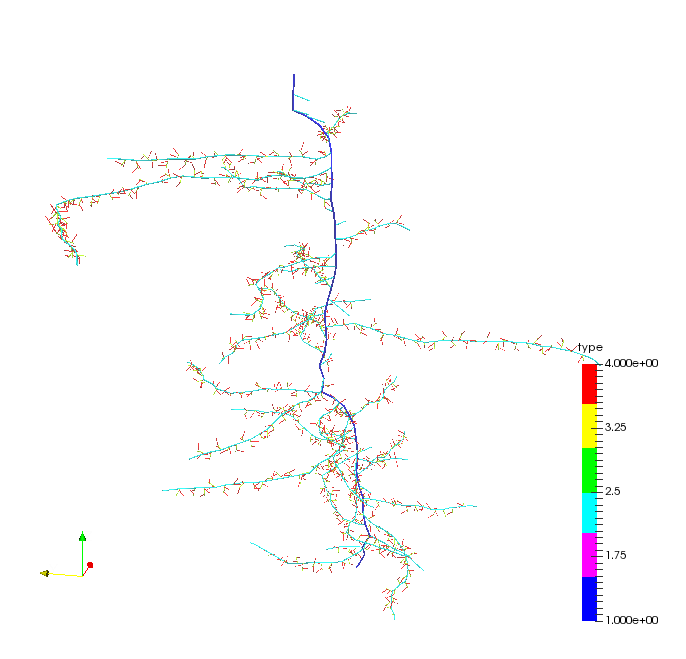
\includegraphics[width=0.99\textwidth]{example_1a.png}
\subcaption{Unconfined growth (Example 1a)} \label{fig:basicA}
\end{subfigure}
\begin{subfigure}[c]{0.5\textwidth}
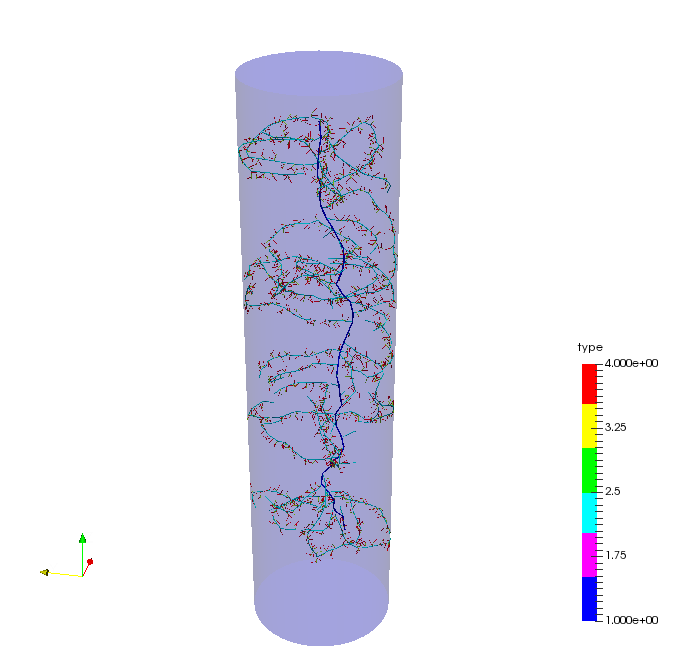
\includegraphics[width=0.99\textwidth]{example_1b.png}
\subcaption{Confined to soilcore (Example 1b)} \label{fig:basicB}
\end{subfigure}
\caption{Paraview visualizations of results of example 1a and 1b.} 
\end{figure}

Next, we show how to build more complex container geometries using SDF, 
furthermore, we show an example with multiple root systems that is computed in parallel.

\subsection{Using SDF with set operations}

In the following example we create geometries that we might encounter in experiments. 
First, we show how to rotate a rhizotron (e.g. to see more roots at the wall due to gravitropism). 
Second, we create a split box experiment, and furthermore, an example where rhizotubes act as obstacles.

The following examples demonstrates how to build a complex geometry using rotations, translations and set operations on the SDF.

\lstinputlisting[language=Python, caption=Example 1c]{../../examples/python/example1c_complexcontainer.py}

\begin{itemize}

\item[15-21] Definition of a rotated rhizotron, see Figure \ref{fig:rhizo}: 
L17 creates the flat container with a small height, this container is then rotated and translated into the desired position. 
L18 is the position where the origin will lie, and L19 the rotational matrix around the x-axis. 
In L20 the origin position is rotated. Finally, in L21 the new rotated and translated geometry is created. 
\item[23-32] Definition of of a split box, see Figure \ref{fig:split}: 
The split box is composed of a left box, a right box, and a top box connecting left and right. 
In L31 the geometry is defined by the set operation union of the three compartments. 
\item[34-49] Definition of rhizotubes as obstacles, see Figure \ref{fig:rhizotubes}: L35 is the surrounding box, 
L36 a single rhizotube, that is rotated around the y-axis in L37. 
L39-L46 create a list of rhizotubes at different locations that mimics the experimental setup. 
L48 and L49 compose the final geometry by to set operation, first a union of all tubes, 
and then cut them out the surrounding box by taking the difference. 
\item[52] Pick one of the three geometries for your simulation.
\item[62] Also more complex geometries can be visualized by the Paraview script, 
however, set operations are not really performed, only the involved geometries are visualized.
\item[65] As before we cannot visualize the container geometry in the interactive rendering, but only the roots. We give two additional arguments: The first argument 'True' indicates that an interactive window should be created, otherwise with 'False' we are only interested in the return value of the method. The second argument is the axis alignhment. Currently, the options are 'top\_view', 'side\_view' (default), or 'oblique'. 

\end{itemize}

% TODO describe the creation of the paraview plots in detail...

\begin{figure}
\begin{subfigure}[c]{0.3\textwidth}
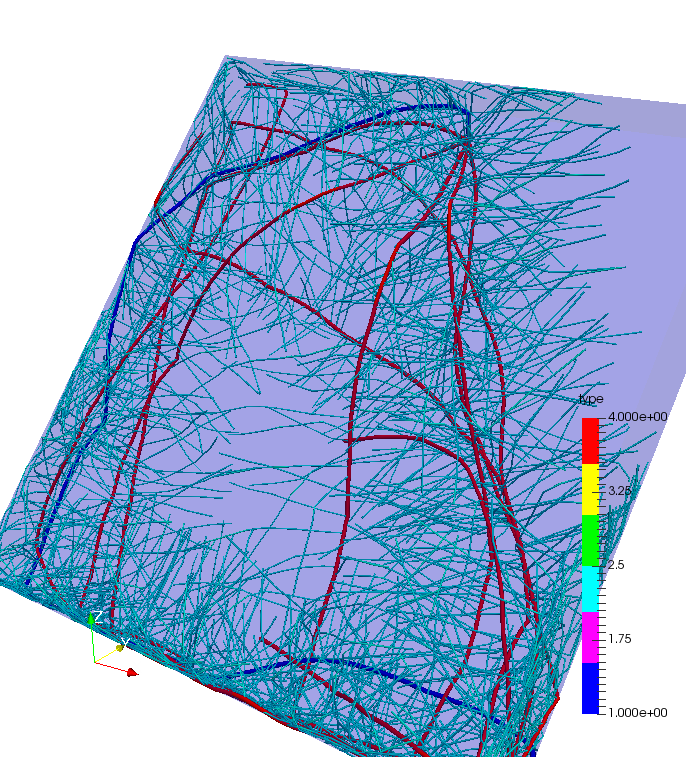
\includegraphics[width=0.99\textwidth]{example_2a1.png}
\subcaption{Rotated rhizotron} \label{fig:rhizo}
\end{subfigure}
\begin{subfigure}[c]{0.3\textwidth}
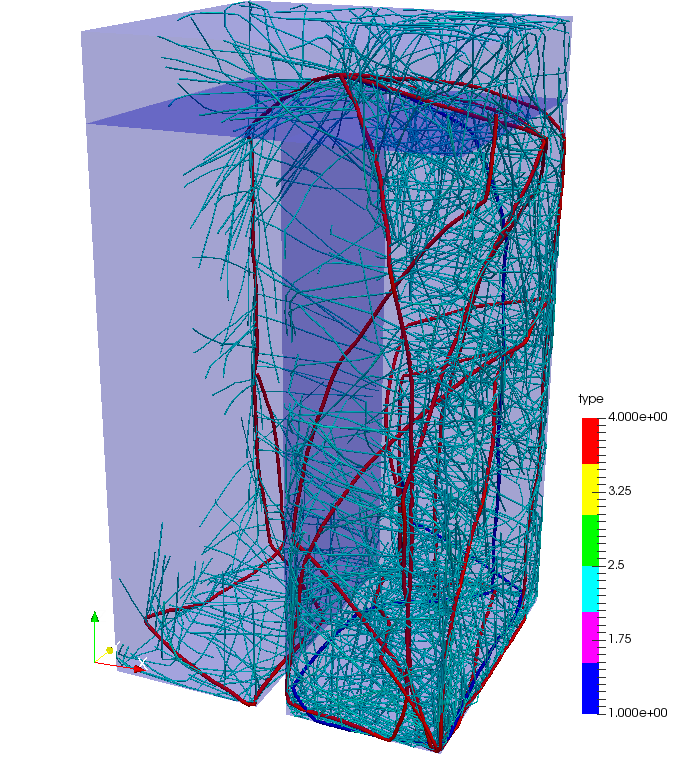
\includegraphics[width=0.99\textwidth]{example_2a2.png}
\subcaption{Split box} \label{fig:split}
\end{subfigure}
\begin{subfigure}[c]{0.3\textwidth}
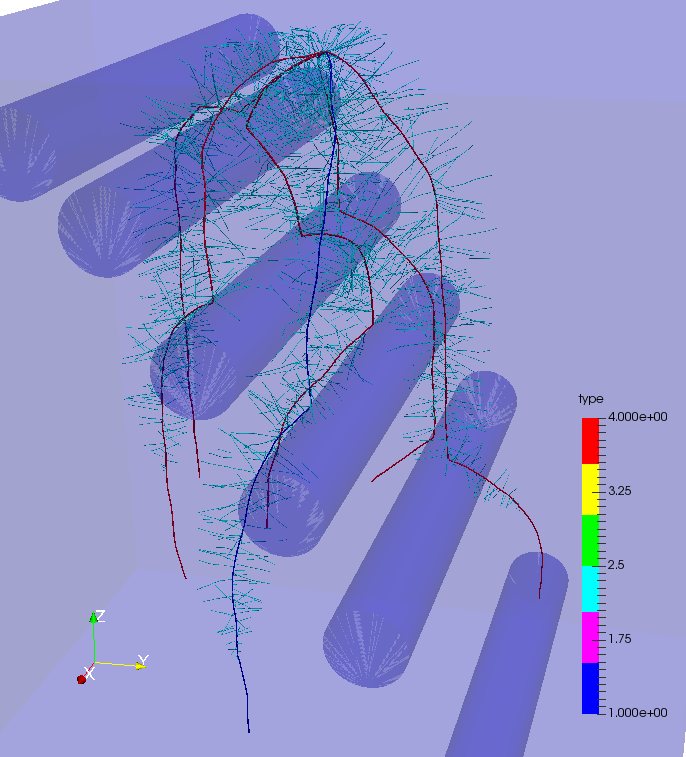
\includegraphics[width=0.99\textwidth]{example_2a3.png}
\subcaption{Rhizotubes} \label{fig:rhizotubes}
\end{subfigure}
\caption{Different geometries described by SDF}
\end{figure}

\subsection{Multiple root systems}

Its possible to simulate multiple root systems. In the following we show a small plot scale simulation.

\lstinputlisting[language=Python, caption=Example 1d]{../../examples/python/example1d_multiple.py}

\begin{itemize}

\item[11,12] Set the number of columns and rows of the plot, and the distance between the root systems.

\item[15-22] Creates the root systems, and puts them into a list allRS. L20 sets the position of the seed. 

\item[25,26] Simulate all root systems 

\item[29-36] Saves each root systems, and additionally, saves all root systems into a single file. 
Therefore, we create an SegmentAnalyser (see Section \ref{sec:sa}) object in L29 and merge all segments into it L33, 
and finally export the single file L36. The resulting geometry is shown in Figure \ref{fig:multiple}.

\end{itemize}

If we consider only one plant type we often simplify plot scale simulations to a single plant simulation with periodic boundary conditions. We can analyse the root geometry with an underlying periodic grid as described in Section \ref{ssec:periodic}. 

\begin{figure}
\centering
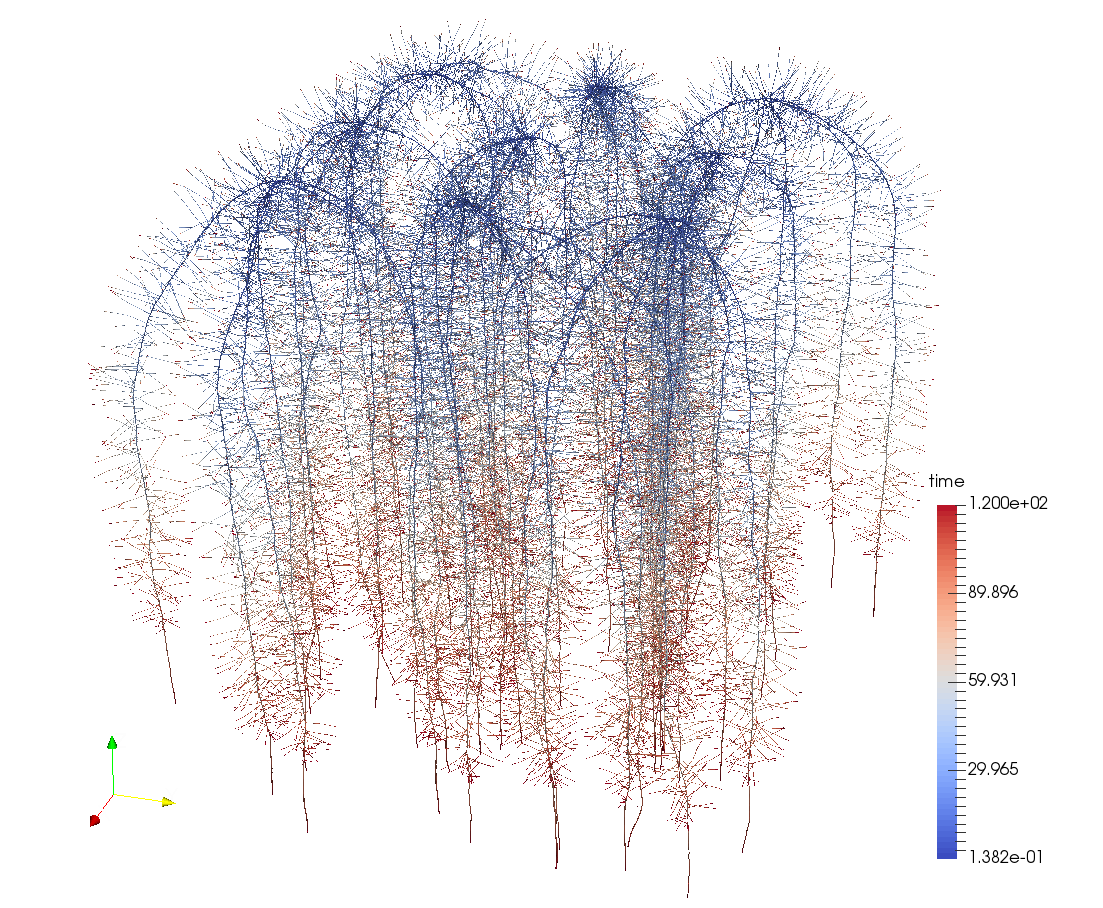
\includegraphics[width=0.7\textwidth]{example_2b.png}
\caption{Multiple root systems, colors denote the creation time of the root segments} \label{fig:multiple}
\end{figure}


\newpage
\section{The RootSystem class} \label{sec:rs}

The class RootSystem is responsible for the model parameters and controls the simulation. Additionally, the class offers utility functions for post processing on a per root level, where each root is represented as a polyline, which is represented by a Python list of nodes. 

Post processing functions per segment can be found in the class SegmentAnalyser (see Section \ref{sec:sa}). A segment is a part of the root and is represented by two nodes that are connected by a straight line.



\subsection{Initialize parameters from scratch} \label{sec:from_scratch}
 
In the previous examples we opened the root system parameters from an xml file. In this example we show how to do everything in a Python script without the need of any parameter file. This is especially important if we want to modify parameters in our scripts (e.g. like it is needed for a sensitivity analysis, see Section \ref{ssec:sensitivity}).

In order to set up a simulation by hand, we have to define all relevant model parameters. This is done by creating a RootRandomParameter object for each root order or root type, and one SeedRandomParameter for each plant type. 

Note that during the simulation, the parameters for a specific root (RootSpecificParameter) are generated from the RootRandomParameter class which represents the random distributions of certain parameters.

\lstinputlisting[language=Python, caption=Example 2a]{../examples/example2a_initializeparams.py}

\begin{itemize}
\item[5] Matplotlib is Python's easy way to create figures like in Matlab.\item[6] NumPy is Python's scientific computing package.

\item[9,10] Create the root type parameters of type 1 and type 2.
\item[12-38] We set up a simple root system by hand. First we define the tap root L12-L26, then the laterals L28-L38. By default all standard deviations are 0. Most parameters standard deviations can be set with an additional 's' appended to the parameter name, e.g. $lmaxs$ is the standard deviation of $lmax$, see L32
\item[40,41] Set the root type parameters.

\item[43-47] Create an object of class SeedRandomParameter which defines when basal and shoot borne roots emerge. In this example we neglect basal and shoot borne roots, and just define the seed location, and deactivate basal roots by setting their maximal number $maxB$ to 0 ($firstB$ and $delayB$ are ignored in that case). 
\item[48] Sets the root system parameters.

\item[53] We choose the simulation times in a way that we can see the temporal development, and that all lateral roots have emerged in the final time step.

\item[54-70] Within the simulation loop we create Figure \ref{fig:ip}. L58-61 defines the limits and titles. In L63 we retrieve the roots as polylines which are represented by a list of nodes. In L64-67 we plot the $x$ and $z$ coordinates for each segment ($n$, $n2$) as green line. 

\item[75-80] It is not only possible to set all model parameter, 
but to retrieve the parameters after the simulation with rs.getParameter(), which returns one value per root. For all parameters that are derived from a random distribution the root specific parameter is returned (e.g. $la$, L78), i.e. the values that were drawn from the normal distribution. The root random parameter can be accessed by adding '\_mean', '\_dev' to the parameter value (e.g. $la\_mean$, L79).

\end{itemize}

Note that all parameters can be set and modified within Python. Especially, standard deviations can be set to zero in order to be able to precisely predict the result. For example we can calculate the total root system length analytically, and check if the numerical simulation yield the (exact) same result. This is performed in the tests test\_root.py, and test\_rootsystem, which is used to test and validate CPlantBox (see folder CPlantBox/test).

With such simple simulations, we can quickly check if the model does, what we expect. For example the maximal number of laterals of above parameters is 16 
$= round(lmax - la - lb)/l_n +  1$. We can calculate the time when the final lateral emerges as $-(lmax/r)*\ln(1-(lmax-l_n/2)/lmax)$ = 122.8 days. At simulation time 125 the last lateral root that has emerged is 2.2 days old, and therefore approximately 4.4 cm long (initial growth rate $r_1 = 2$), which agrees with Figure \ref{fig:ip}.

By default the length of the apical zone is fixed, when the root is created. During growth the apical zone stays in the interval $[la - l_n/2, la+l_n/2]$. The first branch emerges at length $lb$, when the root length reaches $lb +la$.

In the following two subsections we show, how tropism parameters and inter lateral spacing will affect the resulting root system.

\begin{figure}
\centering
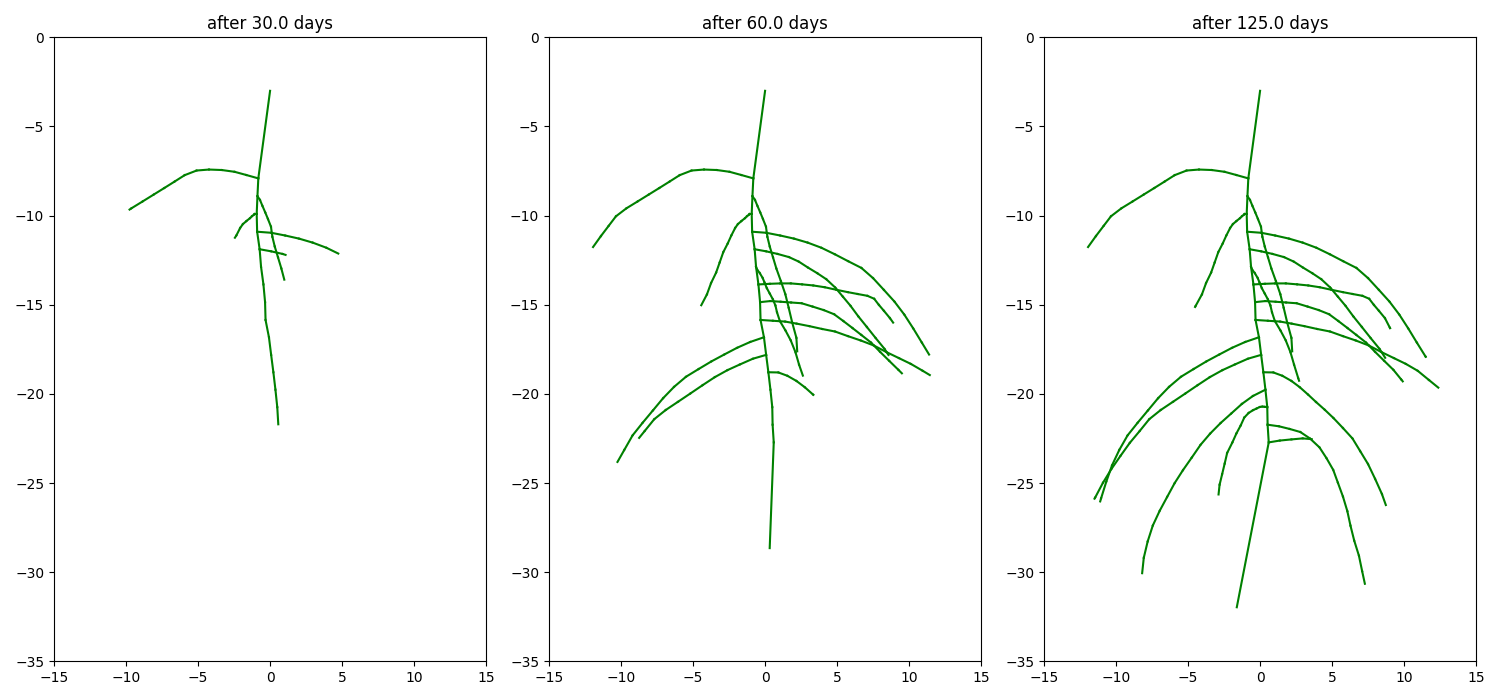
\includegraphics[width=\textwidth]{fig_initializeparams.png}
\caption{Root development} \label{fig:ip}
\end{figure}



\subsection{Root tropism parameters $N$ and $\sigma$} \label{ssec:tropism}

We show the influence of the parameters $N$ and $\sigma$ in the case of gravitropism. The parameter $N$ [1] denotes the strength of the tropism, and $\sigma$ [cm$^{-1}$] the flexibility of the root, i.e. the expected angular variation per cm root length. 

\lstinputlisting[language=Python, caption=Example 2b]{../examples/example2b_tropism.py}

\begin{itemize}
\item[10-13] We choose the parameter values $N$ and $\sigma$ we want to plot. It might be interesting to change the initial insertion $angle$, and the axial resolution $dx$. Note that a change in axial resolution should not qualitatively change the resulting images.

\item[15-18] The root system is created and SeedRandomParameters are set to produce a basal root every third day. 

\item[20-23] The RootRandomParameter for tap and basal roots is defined.

\item[25-28] The loop runs over the parameters we want to modify. We create a subplot for each configuration, and start with a new root system by calling reset in L28.

\item[30-34] We set the parameters (L30,L31) and do the simulation (L33,L34)

\item[36-44] Matplotlib is used for visualization (looping over the segments is rather slow). L36 gives a list of all nodes, and L37 of all segments as two node indices. Therefore, each segment starts at node n1 and ends at node n2, as defined in L39.

\item[L48] Creates Figure \ref{fig:tropism}.
\end{itemize}

In the first column ($\sigma$=0) of Figure \ref{fig:tropism} nothing happens, because if the root has no flexibility to bend, the strength has no influence on the resulting root system. The first row ($N$=0) shows the influence of $\sigma$ only. The growth is undirected, because the strength of the gravitropism is zero. If the roots have small flexibility, they grow downwards because they initially do. 

The other subplots show different shapes of the root system. We normally derive the two parameters $N$ and $\sigma$ by visual comparison. Note that results are independent of the root axial resolution $dx$ and the temporal resolution.

\begin{figure}
\centering
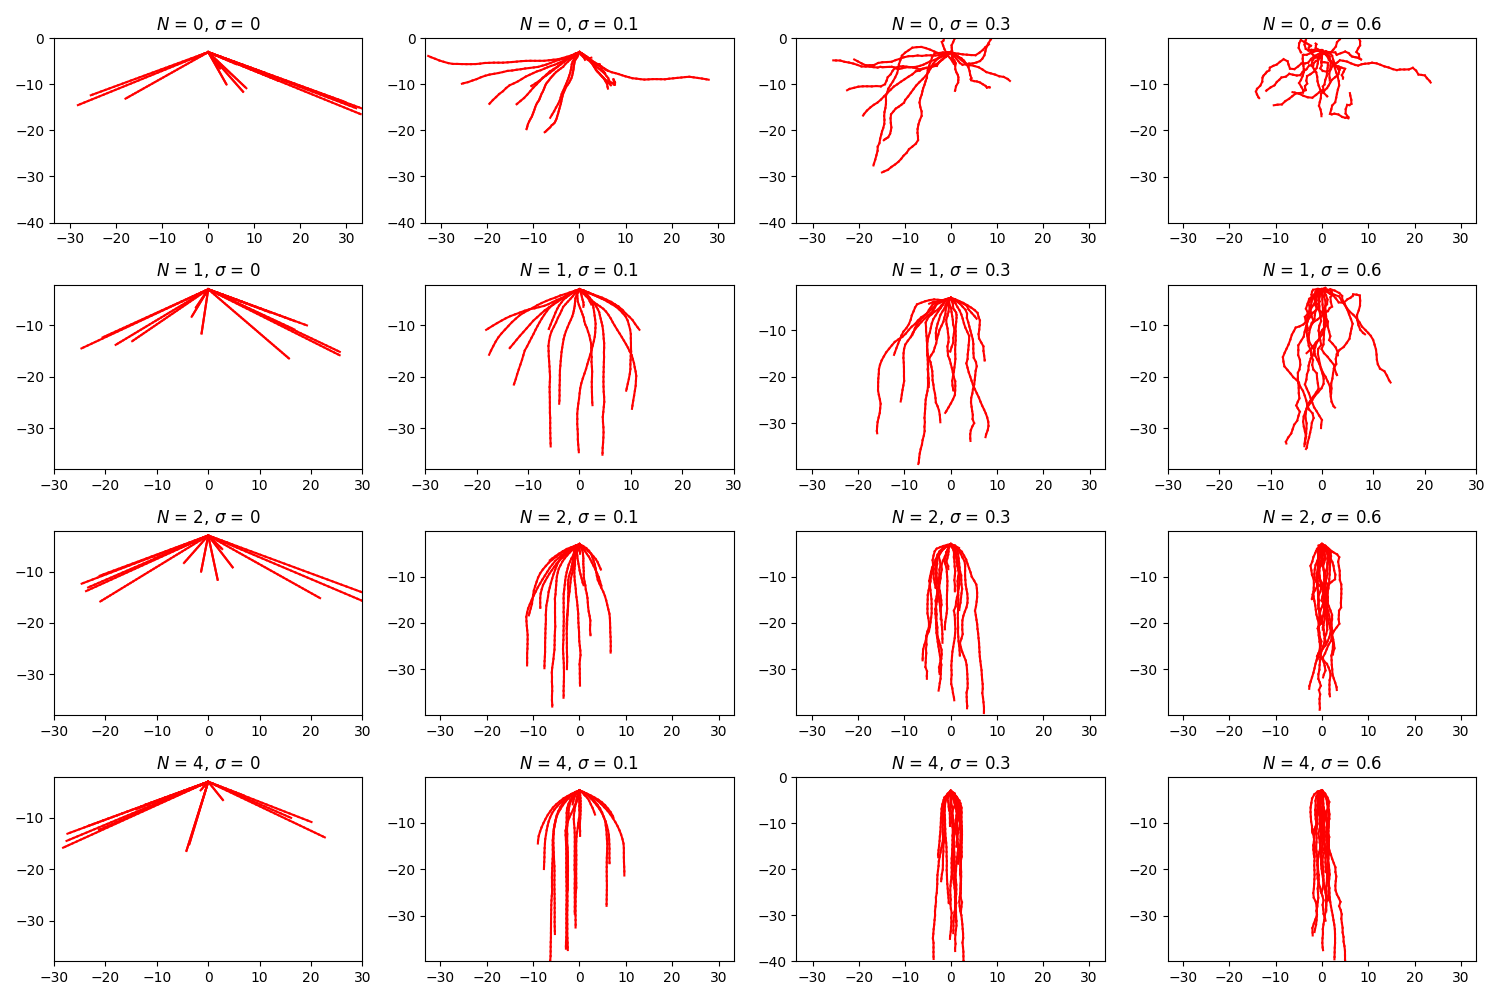
\includegraphics[width=\textwidth]{fig_gravitropism.png}
\caption{Influence of $N$ and $\sigma$ in case of gravitropism} \label{fig:tropism}
\end{figure}




\subsection{Inter lateral spacing ($ln$, $lnk$)} \label{ssec:spacing}

A single root is divided in basal zone, root branching zone, and root apical zone. Basal and apical zone are given by the parameters $la$, and $lb$ with standard deviations $la_s$ and $lb_s$. The branching zone has the size $lmax-la-lb$, where $lmax$ is the maximal root length. The branching zone is divided into inter lateral distances $l_n$, which are values drawn from a normal distribution with standard deviation $l_{ns}$. All values are fixed when the root is created This is performed in the method RootRandomParameter::realize(). The chosen parameters reflect the root growth under perfect conditions. Based on this, the root development can then be influenced by environmental conditions e.g. impeding growth speed, or lateral emergence, see Section \ref{sec:functional}.

Normally, the setting constant branching distances is sufficient, but sometime experimental data indicate that inter lateral distances are smaller, or larger near the base than near the root tip. The reason for this could be soil root interaction (e.g. root response to dense or nutritious layer), or within the genotype. We added a purely descriptive parameter to mimic such experimental observations. The parameter $lnk$, which is zero per default, defines the slope, at the mid of the branching, altering the inter lateral distance linearly along the root axis. In the following script, we demonstrate the usage of $lnk$.

\lstinputlisting[language=Python, caption=Example 2c]{../examples/example2c_lateralspacing.py}

\begin{itemize}
\item[10-13] A root system with a single tap root is created. 
\item[16,16] The axial resolution, and insertion angle is defined. We take a very large axial resolution for the tap root, since we visualize the nodes later on, and we want to see only lateral branching nodes.
\item[18-24] Definition of the tap root. Standard deviations are zero, we do not want any variations. Tropism parameters are chosen in a way, that the tap root grows straight downwards.
\item[26-29] Definition of the first order lateral. Tropism is a strict exotropism (i.e. root follows its initial growth direction).
\item[31,32] The parameter values we want to visualize.
\item[36] Resets the root system (to $simTime = 0$). Root parameters are not changed. 
\item[38,39] Sets the values for this subplot. 
\item[41,42] Runs the simulation
\item[44-56] Creates the subplots. First (L47-49) we plot all segments in green. And second (L51-53) we plot all nodes of the tap root as red asterisks.
\item[58-60] Creates Figure \ref{fig:spacing}
\end{itemize}

The mid column of Figure \ref{fig:spacing} shows to different inter lateral distances, 4 (top) and 2 (cm) bot. The left column demonstrate the use of negative values for $lnk$ which results in larger distances near the base. The right column has positive values for $lnk$, which will result in smaller distances near the base. The $i$-th inter distance is calculated as $ln_i = ln + lnk (x_i-mid_x)$, where $x_i$ is the position within the branching zone, and $mid_x$ is the mid of the branching zone. This is done in RootRandomParameter::realize(). Note that $lnk$ is dimensionless and the slope in the linear equation. At mid of the branching zone the inter-lateral distance equals $ln$. 

\begin{figure}
\centering
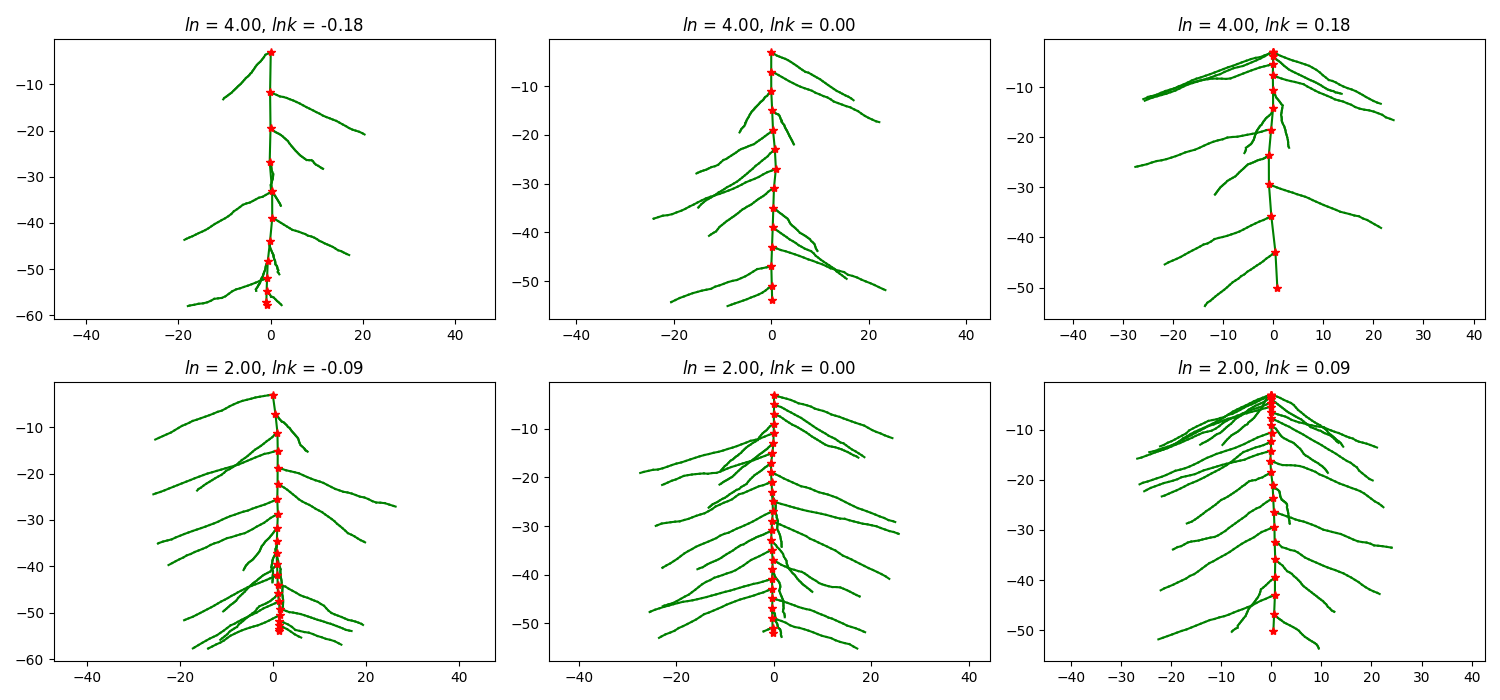
\includegraphics[width=0.99\textwidth]{fig_lateralspacing.png}
\caption{Inter-lateral spacing, larger near base (left column), constant (mid column), and smaller near base (right column) } \label{fig:spacing}
\end{figure}

In the following we show, how to analyse model results on a per root basis using the RootSystem class. To create density distributions the resulting root segments are analysed using the SegmentAnalyser class, described in Section \ref{sec:sa}.


\subsection{Root system length over time}

The following script shows how to analyse root system length versus time. 

\lstinputlisting[language=Python, caption=Example 2d]{../examples/example2d_length.py}

\begin{itemize}
\item[9-14] Sets up the simulation.

\item[16-18] Defines the simulation time, time step, and the resulting number of simulate(dt) calls. 

\item[21] First we state which scalar type we want to analyse ('volume', 'surface', or 'one' would also make sense). 

\item[22] Pre-definition of the numpy arrays storing the lengths over time. 

\item[23-30] The simulation loop executes the simulation for a single time step L24. L25 calculates the type of each root (the organ subType), L26 the length (or any other parameter) of the root. L27-L30 calculates the total root length at the current time step for all roots, and for specific root types. The method rs.getParameter collects this data from the RootSystem organs. It is possible to access all root random parameters and resulting realisations using rs.getParameter. In C++ the class functions are defined in Root::getParameter, Organ::getParameter. 

\item[32-38] Creates Figure \ref{fig:length}.

\end{itemize}



\subsection{Root tips and root bases}

Next we show two options how to retrieve root tip and root base positions from a simulation:

\lstinputlisting[language=Python, caption=Example 2e]{../examples/example2e_roottips.py}

\begin{itemize}

\item[14,15] Reset the simulation and simulate for only 7 days (otherwise there are so many root tips).

\item[17-18] Outputs the number of nodes and segments to get an idea how big the resulting root system is. 
Note that number of segments equals the number of nodes minus the number of base roots that will emerge. 
Base roots are tap roots, basal roots and shootborne roots.

\item[20-26] The first approach retrieves all roots as polylines L21. 
Root tips are the last nodes of the polylines L26, root bases the first nodes L25. Roots that have not started to grow have only 1 node, and are not retrieved by getPolylines().

\item[28-31] Second approach: L29 rs.getNodes() returns all nodes of the root system as a list of nodes, i.e. Vector3d objects. Each Vector3d object can be converted into a numpy array automatically, but is necessary to do that for each element of the list. The methods L30, L31 return the indices of the tips and bases. 

\item[33-41] Creates Figure \ref{fig:scatter} using the second approach.

\item[44,45] Verifies that both approaches yield the same result.

\end{itemize}

\begin{figure}
\begin{subfigure}[c]{0.5\textwidth}
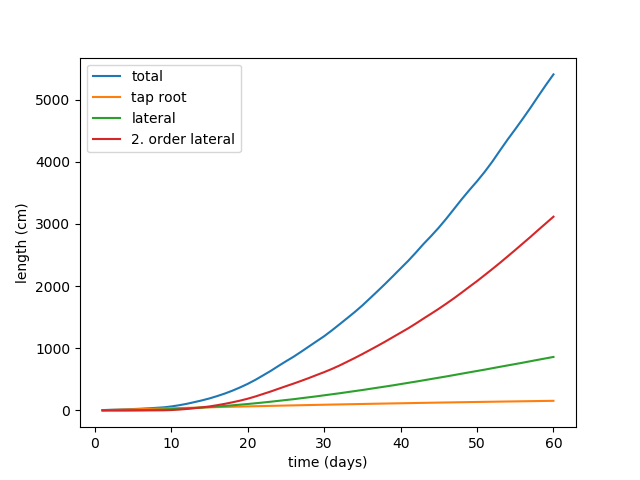
\includegraphics[width=0.99\textwidth]{example_3a.png}
\subcaption{Total root length versus time} \label{fig:length}
\end{subfigure}
\begin{subfigure}[c]{0.5\textwidth}
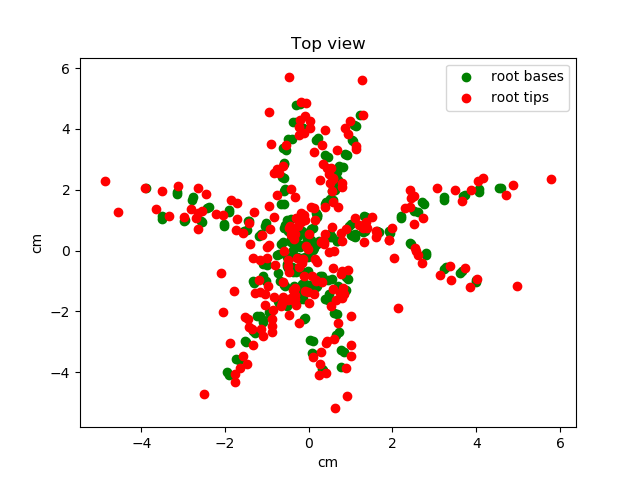
\includegraphics[width=0.99\textwidth]{example_3b.png}
\subcaption{Top view of the root tip and root bases} \label{fig:scatter}
\end{subfigure}
\caption{Root system analysis: Example 2d (a), Example 2e (b)} 
\end{figure}



\subsection{Sensitivity analysis} \label{ssec:sensitivity}

In the next part we vary given parameters in order to make a sensitivity analysis. This takes a lot of simulation runs, and we demonstrate the of use parallel computing to speed up execution.

In this exemplary sensitivity study we will vary the insertion angle of the tap and basal root, and look at the resulting change in mean root tip depth and root tip radial distance. 

\lstinputlisting[language=Python, caption=Example 2f]{../examples/example2f_sensitivity.py}

\begin{itemize}

\item[12-20] Defines a function to set all standard deviations proportional to the parameter values. We use this function in the following to set the standard deviation to zero everywhere. 

\item[23-29] Parameters of the analysis. $N$ denotes the resolution of the parameter we vary, and $runs$ the number of iterations, i.e. a total of $N\cdot runs$ simulations are performed. In L29 we define the insertion angle to be varied linearly between 0 and $\pi/2$.

\item[33-52] Definition of a function that performs the simulation and returns mean root tip depth and radial distance. First we create a root system and set the standard deviation to zero L34-L36. L37, amd L39 sets the insertion angle. L41 initializes the root system and states that basal root are of root type 1 (same as tap root). The False value turns of verbosity to avoid any outputs to the console. L42 performs the simulation. L44-L51 calculates the mean root tip depth and radial distance. 

\item[55-73] This section performs the computation of all simulation runs. L55-56 preallocates the resulting arrays. L62-L68 performs the parallel computations, index $i$ is the index of the insertion angle. L71-73 calculates the mean values per simulation run.

\item[74-83] Creates the resulting Figure \ref{fig:sensitivity}. Note that the resulting curves become smoother, if the number of runs is increased (L28).

\end{itemize}

\begin{figure}
\centering
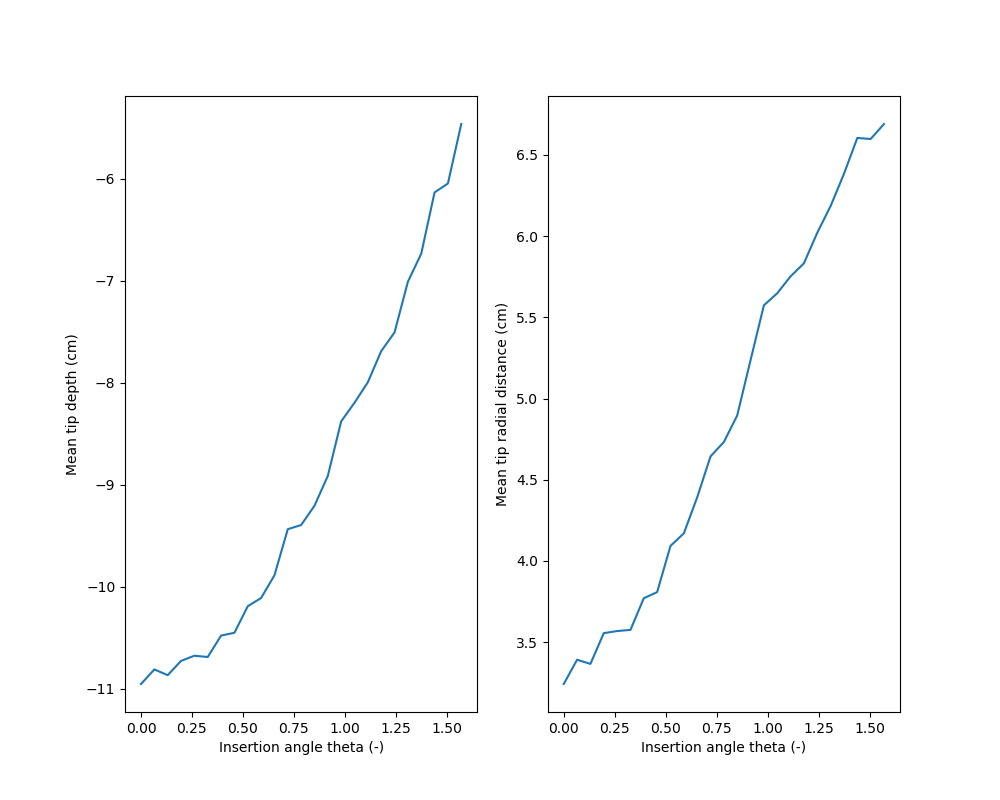
\includegraphics[width=0.7\textwidth]{example_4b.png}
\caption{Sensitivity of mean root tip depth (left) and radial distance (right) to the insertion angle theta (Example 2f) } \label{fig:sensitivity}
\end{figure}


\newpage
\section{The SegmentAnalyser class} \label{sec:sa}

The class SegmentAnalyser offers post-processing methods per root segment. The advantage is that we can do distributions or densities, and that we can analyse the segments within any geometry. 

We start with a small example plotting the root surface densities of a root system versus root depth.

\subsection{Root surface densities}

\lstinputlisting[language=Python, caption=Example 3a]{../examples/example3a_density.py}

\begin{figure}
\centering
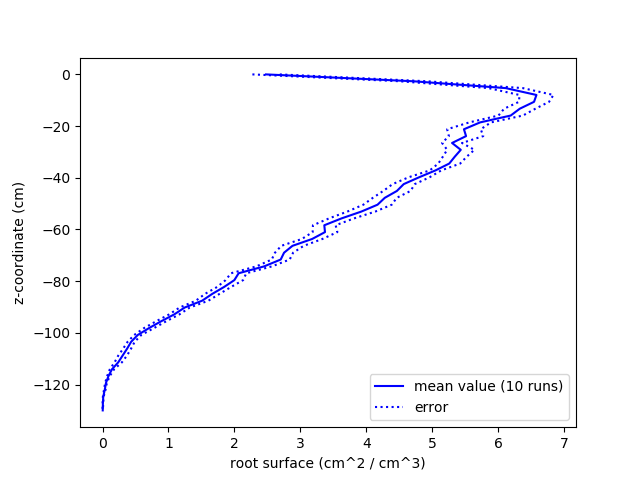
\includegraphics[width=0.7\textwidth]{example_3c.png}
\caption{Root surface densitiy versus depth(Example 3a)} \label{fig:surface_density}
\end{figure}


\begin{itemize}

\item[8-12] Pick a root system.
\item[14-16] Depth describes the y-axis of the graph, layers the number of vertical soil layers, where the root surface is accumulated, and runs is the number of simulation runs. 
\item[18-23] Performs the simulations. L23 creates a distribution of a parameter (name) over a vertical range (bot, top). The data are accumulated in each layer, segments are either cut (exact = True) or accumulated by their mid point (exact = False). 
\item[25] In order to calculate a root surface density from the summed up surface, we need to define a soil volume. The vertical height is the layer length, length and width (here 10 cm), can be determined by planting width, or by a confining geometry. 
\item[26-28] Calculates the densities mean and the standard error. 
\item[30-39] Prepares the plot (see Figure \ref{fig:surface_density}).

\end{itemize}



\subsection{Analysis per segment within a geometry}

The following script demonstrates some of the post processing possibilities by setting up a virtual soil core experiment (see Figure \ref{fig:soilcoreGeom}), where we analyse the content of two soil cores located at different positions.

\lstinputlisting[language=Python, caption=Example 3b]{../examples/example3b_sdfanalysis.py}

\begin{itemize}

\item[11-15] Performs the simulation.

\item[17-22] We define two soil cores, one in the center of the root and one 10 cm translated. In L22 we pick which one we use for the further analysis. Figure \ref{fig:soilcoreGeom} shows the resulting geometry, with a soil core radius of 10 cm.

\item[24-28] Prepares three sub-figures. 

\item[31-41] Creates a root length distribution versus depth at different ages. L33 creates the SegmentAnalyser object, and L34 crops it to a fixed domain or maps it into a periodic domain. In L38 the filter function keeps only the segments, where the parameter (first argument) is in the range between second and third argument. L39 creates the distribution. 

\item[44-54] We repeat the procedure, but we crop to the soil core selected in L22. 

\item[57-89] In the third sub plot we make densities of specific root types like basal roots, first order roots, and second order roots. In L58 we crop the segments to the soil core geometry. In L63 we filter for the selected sub type, and in L64 we create the density distribution.

\item[71-73] Show and save resulting Figure \ref{fig:central} and \ref{fig:shifted} for the two soil cores (chosen in L22).

\end{itemize}

\begin{figure}
\centering
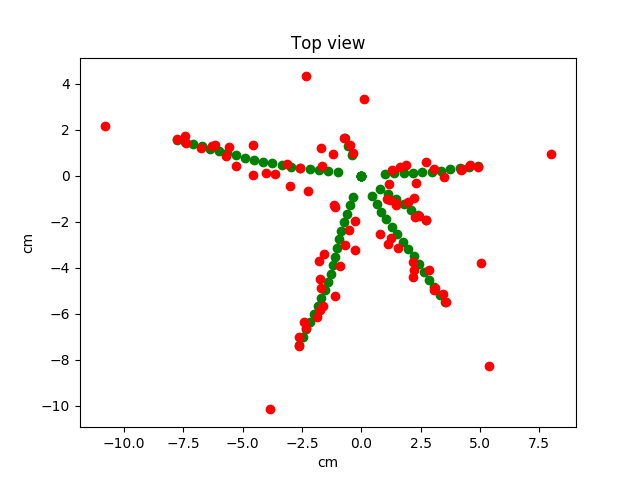
\includegraphics[width=0.7\textwidth]{example_3d.png} % 
\caption{Virtual soil cores experiment (Example 3b): Central core (blue), shifted core (red)} \label{fig:soilcoreGeom}
\end{figure} 


The example shows differences between the central core and shifted core (see Figure \ref{fig:central} and \ref{fig:shifted}) because the central core captures all roots emerging from the seed. The basic idea is that such analysis can help to increase the understanding of variations in experimental observations.

\begin{figure}
\centering
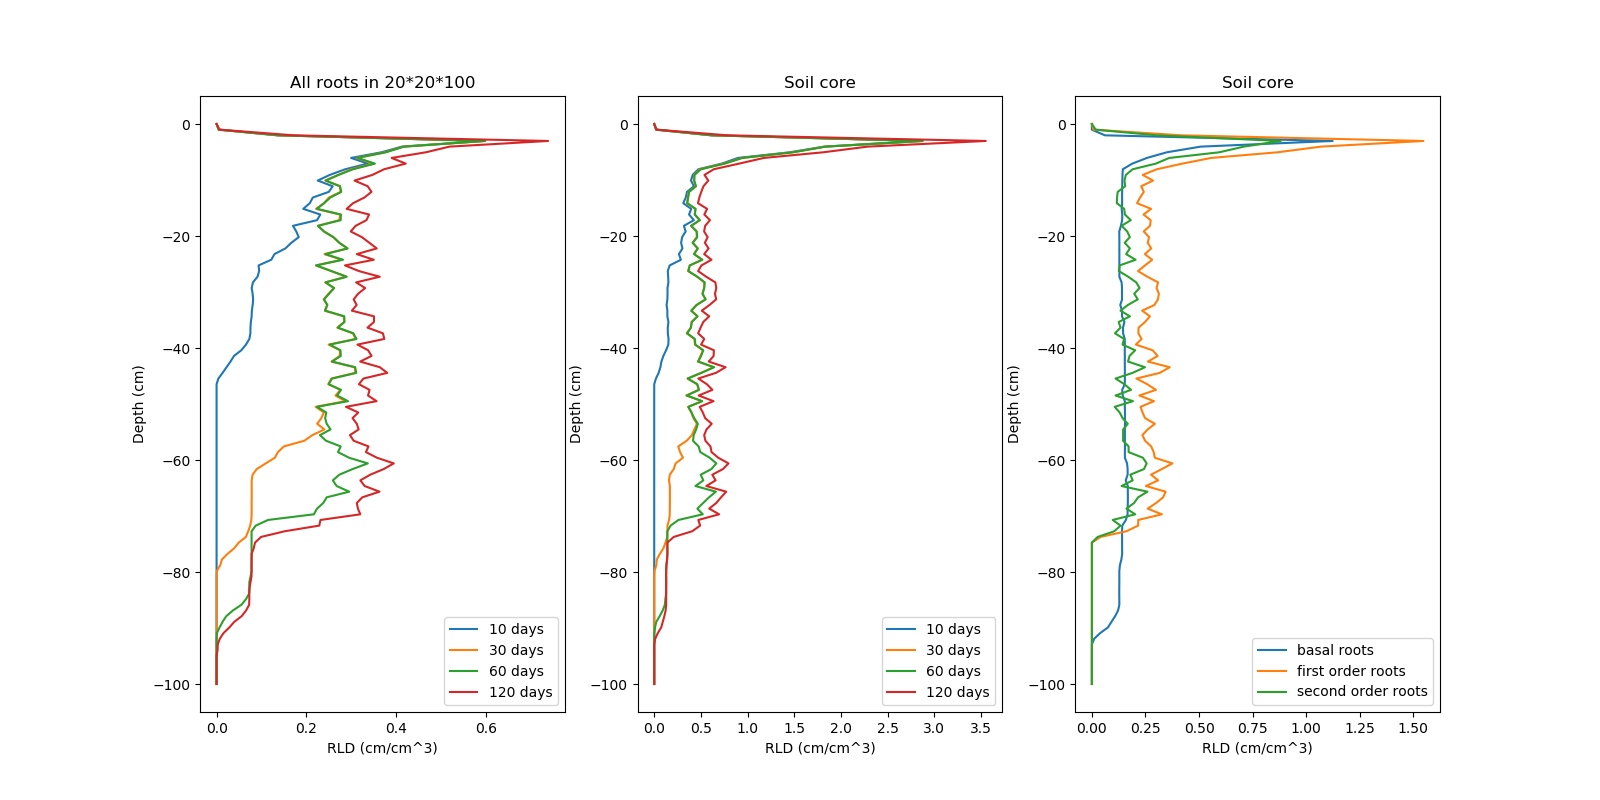
\includegraphics[width=0.9\textwidth]{example3b.png} 
\caption{Central core (Example 3b)} \label{fig:central}
\end{figure}

\begin{figure}
\centering
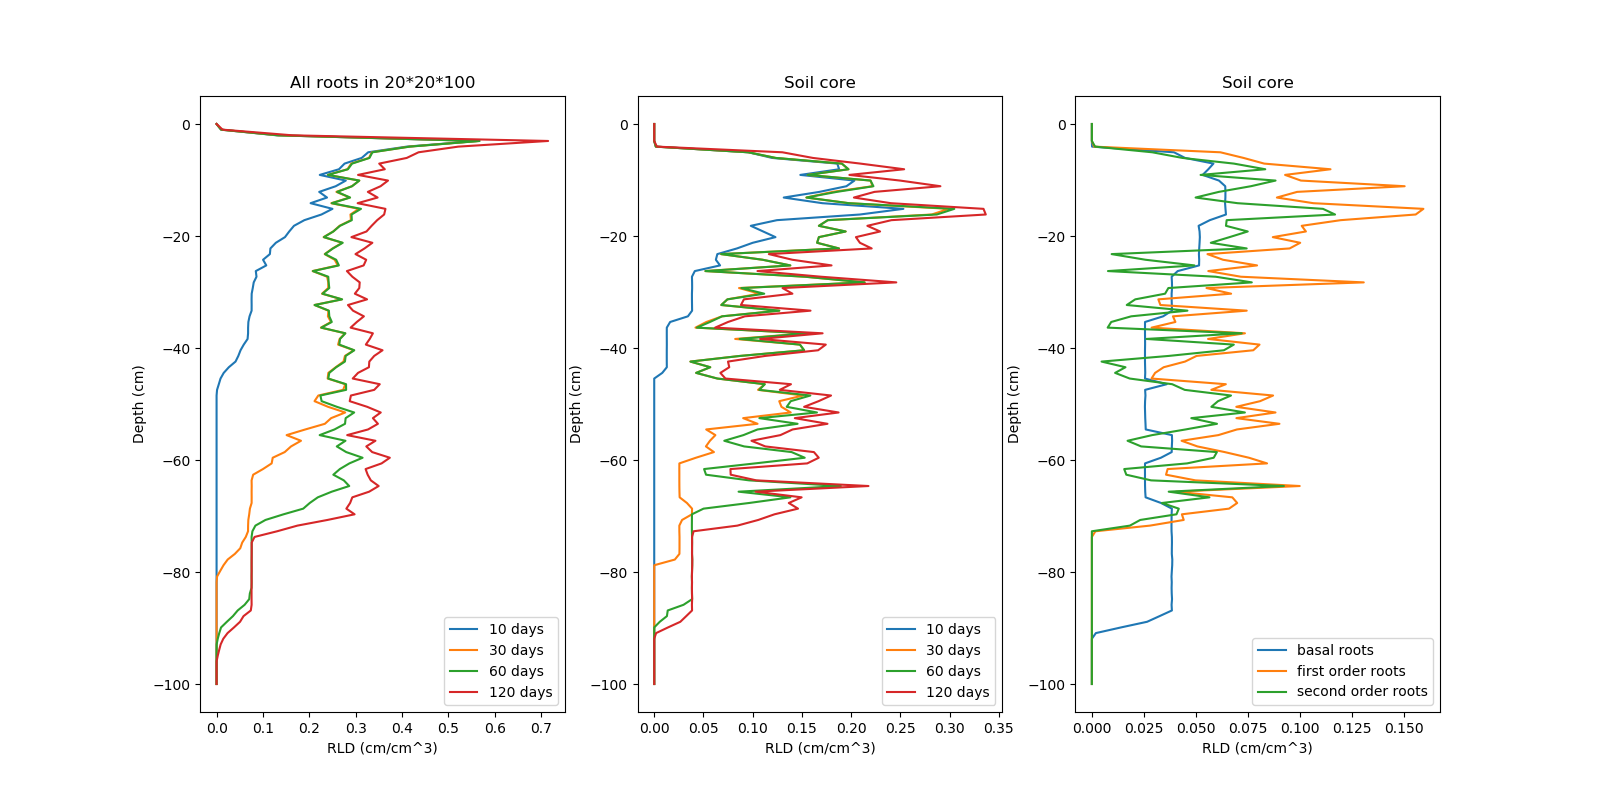
\includegraphics[width=0.9\textwidth]{example3b2.png} 
\caption{Shifted core (Example 3b)} \label{fig:shifted}
\end{figure}


\subsection{SegmentAnalyser for DGF or VTP export}

If we want to export our root system as dune grid file (dgf) we need to introduce an artificial shoot. By default the tap root and basal root starts at the seed node (i.e. multiple segments start at the same node), and its difficult to define a boundary condition for such a situation (e.g. in DuMux). Furthermore, if there are shoot borne roots, they emerge out of nothing above the seed node. Therefore, we introduce artificial segments eventually connecting shoot borne roots (if there are any) and connecting the seed node that is normally located at (0,0,-3) to the origin at (0,0,0). The following code snippet shows how to export a root system as dgf file:

\lstinputlisting[language=Python, caption=Example 3c]{../examples/example3c_write.py}

\begin{itemize}
 \item[6-11] Defines a root sytem
 \item[13] Create the analyser object
 \item[15-18] Get the artificial shoot segments from the root system (L15) and manually add them to the SegmentAnalyser (L18), first argument is the segment $s$, second is creation time, third is radius, and fourth arguments states that the segment is inserted at the top of the list (True), while (False) would append it to segment list.
 \item[19] Write the VTP file. For VTP files its possible to add a list of parameters that will be exported. 
 \item[20] Write the DGF file. The parameters are fixed (see documentation of SegmentAnalyser::writeDGF)
\end{itemize}

It is also possible to make use of the SegmentAnalyser class without any other CPlantBox classes (e.g. for writing vtp from measurements). The following example shows how to construct the class with arbitrary nodes and segments (e.g. from measurements). 

\lstinputlisting[language=Python, caption=Example 3d]{../examples/example3d_measurements.py}

\begin{itemize}
 \item[6-9] Define some segments with data
 \item[12,13] We convert the Python list to lists of C++ types
 \item[16] We create the SegmentAnalyser object without an underlying Organism
 \item[18,19] Use the Analyser object, by printing information, or writing a vtp. 
\end{itemize}

Next, we describe how to make an animation from a CPlantBox simulation.


\subsection{How to make an animation} \label{ssec:animation}

In order to create an animation in Paraview we have to consider some details. The main idea is to export the result file as segments using the class SegmentAnalyser. A specific frame is then obtained by thresholding within Paraview using the segments creation times. In this way we have to only export one vtp file. 

We modify example1b.py to demonstrate how to create an animation.

\lstinputlisting[language=Python, caption=Example 4c (modified from Example 1b)]{../examples/example3e_animation.py} 

\begin{itemize}

\item[11,12] Its important to use a small resolution in order to obtain a smooth animation. L18 set the axial resolution to 0.1 cm. 

\item[19,29] Instead of saving the root system as polylines, we use the SegmentAnalyser to save the root system as segments.

\item[22,23] It is also possible to make the root system periodic in the visualization in $x$ and $y$ direction to mimic field conditions.

\item[26-28] We save the geometry as Python script for the visualization in ParaView.

\end{itemize}

After running the script we perform the following operations Paraview to create the animation:
\begin{enumerate}
 \item Open the .vtp file in ParaView (File$\rightarrow$Open...), and open tutorial/examples/python/results/example\_3e.vtp.
 \item Optionally, create a tube plot with the help of the script tutorial/pyscript/rsTubePlot.py (Tools$\rightarrow$Python Shell, press 'Run script').
 \item Run the script tutorial/pyscript/rsAnimate.py (Tools$\rightarrow$Python Shell, press 'Run script'). The script creates the threshold filter and the animation. 
 \item Optionally, visualize the domain boundaries by running the script tutorial/examples/python/results/example\_4e.py (Tools$\rightarrow$Python Shell, press 'Run script'). Run after the animation script (otherwise it does not work).  
 \item Use File$\rightarrow$Save Animation... to render and save the animation. Pick quality ($<$100 \%), and the frame rate in order to achieve an appropriate video length, e.g. 300 frames with 50 fps equals 6 seconds. The resulting files might be uncompressed and are very big. The file needs compression, for Linux e.g. ffmpeg -i in.avi -vcodec libx264 -b 4000k -an out.avi, produces high quality and tiny files, and it plays with VLC.
\end{enumerate}




 

\newpage
\section{Tropisms} \label{sec:tropism}

The change in root growth direction is described by tropisms. In the following we show how to implement directed growth toward higher water content or nutrient concentration, and demonstrate how to simply make new user defined tropism rules. 


\subsection{Hydro- and chemotropism} \label{sec:hydro}

Root growth direction is influenced by soil conditions such as water content, soil strength, or nutrient concentration. In the following example we model the influence of a nutrient rich layer to root system development

\lstinputlisting[language=Python, caption=Example 4a]{../../examples/python/example4a_hydrotropism.py}

\begin{itemize}

\item[6-9] Creates the root system and opens the parameter file

\item[12-17] Change the tropism for all root types: L13 modifies the axial resolution, L14 set the tropism to hydrotropism, and L15-16 sets the two tropism parameters. The parameter $\sigma$ is set to 0.4 for the tap root ($subType$ = 1), and to 1. for the rest of the root types.

\item[19-25] Definition of a static soil property using SDF. We first define the geometry (L20-L21), and then create a static soil (L22) that obtains the maximal value $maxS$ inside the geometry, 
$minS$ outside the geometry, and linear slope with length $slope$. At the boundary the soil has the value $(maxS+minS)/2$.

\item[28] Sets the soil. Must be called before RootSystem::initialize()

\item[41] Initializes the root system, and among others sets up the hydrotropism. 

\item[33-39] Simulation loop

\item[42] Exports the root system geometry

\item[45-46] We actually do not wish to set this geometry, but we abuse the writer of the class RootSytem to export a Python script showing the layer geometry. The resulting ParaView visualization is presented in Figure \ref{fig:chemo}.

\end{itemize}

\begin{figure}
\centering
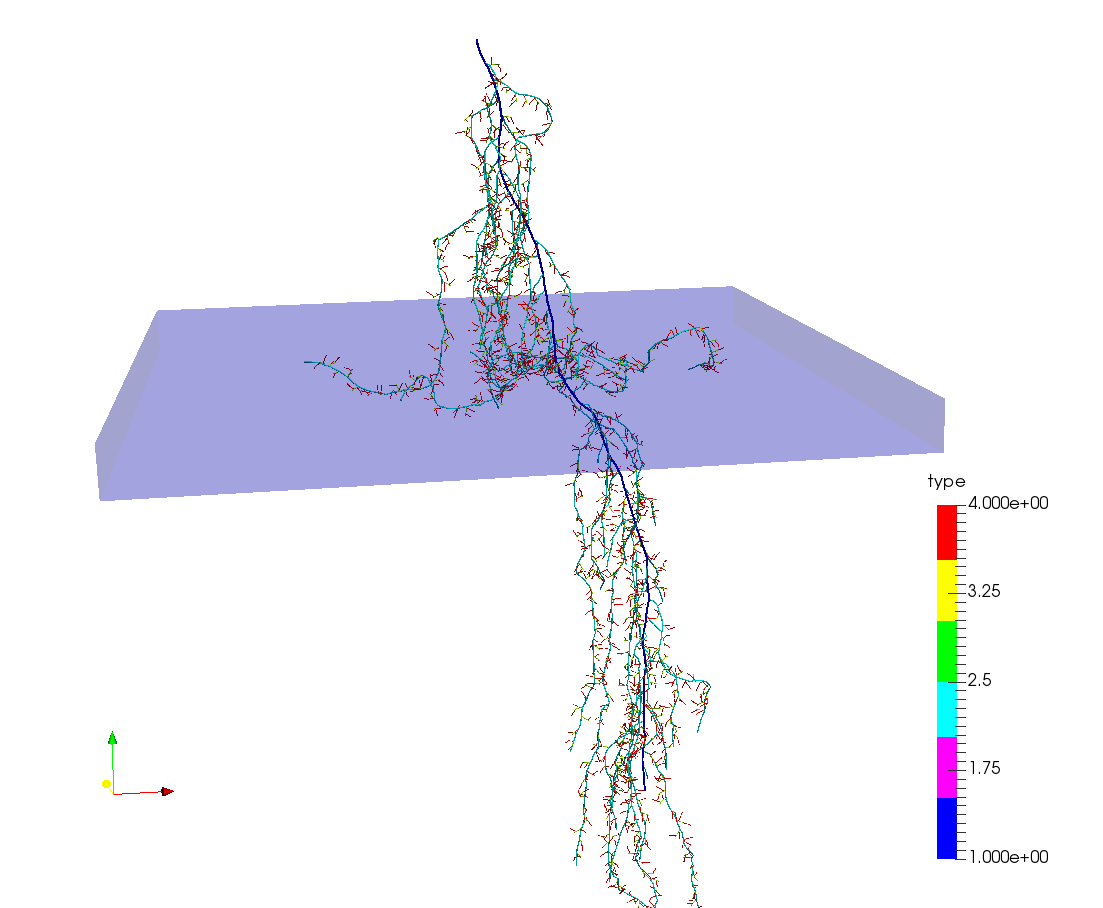
\includegraphics[width=0.7\textwidth]{example4a.png}
\caption{Chemotropism in a nutrient rich layer (Example 4a)} \label{fig:chemo}
\end{figure}



\subsection{Root age dependent growth} \label{sec:usertropism}

Normally, the simulation is created from a set of parameters. For tropisms these are the type of tropism $T$, number of trials $N$ , and tortuosity $\sigma$. There are only a few predefined tropisms called 'gravi', 'plagio', 'exo', or 'hydro', but it is simple to add user defined tropisms.
The following example demonstrates how to define a root age dependent tropism, where roots first grow according to exotropism (following the inital growth direction), and after a certain age change to gravitropic growth.

The new tropism class must be derived from the class Tropism. In CPlantBox tropism is realised with a random optimization process, where the 'best' direction is chosen from $N$ possible direction, according to an objective function that is minimized. Normally, it is sufficient to overwrite this function, called Tropism ::tropismObjective, to change the tropism behaviour. This can be done in Python or in C++. The classes Hydrotropism, Gravitropism, and Plagiotropism (in tropisms.h) are examples for this procedure.

If the whole concept of random optimization is altered, Tropism ::getUCHeading must be overwritten, which is only possible in C++. If the geometry model is also changed Tropism::getHeading must be overwritten.

The following example shows how to implement a new tropism in Python. Two new tropism are introduced:
The first does nothing but to output the incoming arguments of the method Tropism::tropismObjective to the command line (e.g. for debugging). The second one describes a root age dependent tropism that starts with exotropism and changes with root age to gravitropism.

\lstinputlisting[language=Python, caption=Example 4b]{../../examples/python/example4b_usertropism.py}

\begin{itemize}

\item[8-19] Creates a new tropism that just writes incoming arguments of Tropism ::tropismObjective to the command line. This can be used for debugging. The new class is extended from rb.Tropism, and the method Tropism ::tropismObjective is overwritten with the right number of arguments.

\item[22-37] Again, we extend the new class from rb.Tropism. In L25-30 we define our own constructor. Doing this two things are important: (a) the constructor of the super class must be called (L26), and (b) the tropism parameters $n$, and $\sigma$ must be set (L29). 
Furthermore, the constructor defines two tropisms: exo- and gravitropism, that are used in Tropism::tropismObjective at a later point, and a root age that dermines when to switch betwee exo- and gravitropism. \\
In L32-L37 the method Tropism::tropismObjective is defined. We choose the predefined objective function depending on the root age.

\item[41-45] Sets up the simulation.

\item[48-51] L48,L49 creates the first user defined tropsim. Since we did not define a constructor Tropism::setTropismParameter must be called. L50 creates the second user defined tropism.  In L51 the tropism is chosen, using the method Tropism::setTropism. The second argument states for which root type it applies. 
Number 4 is the (default) root type for basal roots, -1 states that the tropism applies for all root types (default = -1).

\item[54-58] The simulation loop. 

\item [61] Exports the result producing Figure (\ref{fig:tropism}). 

\item [64] VTK plot.

\end{itemize}

\begin{figure}
\centering
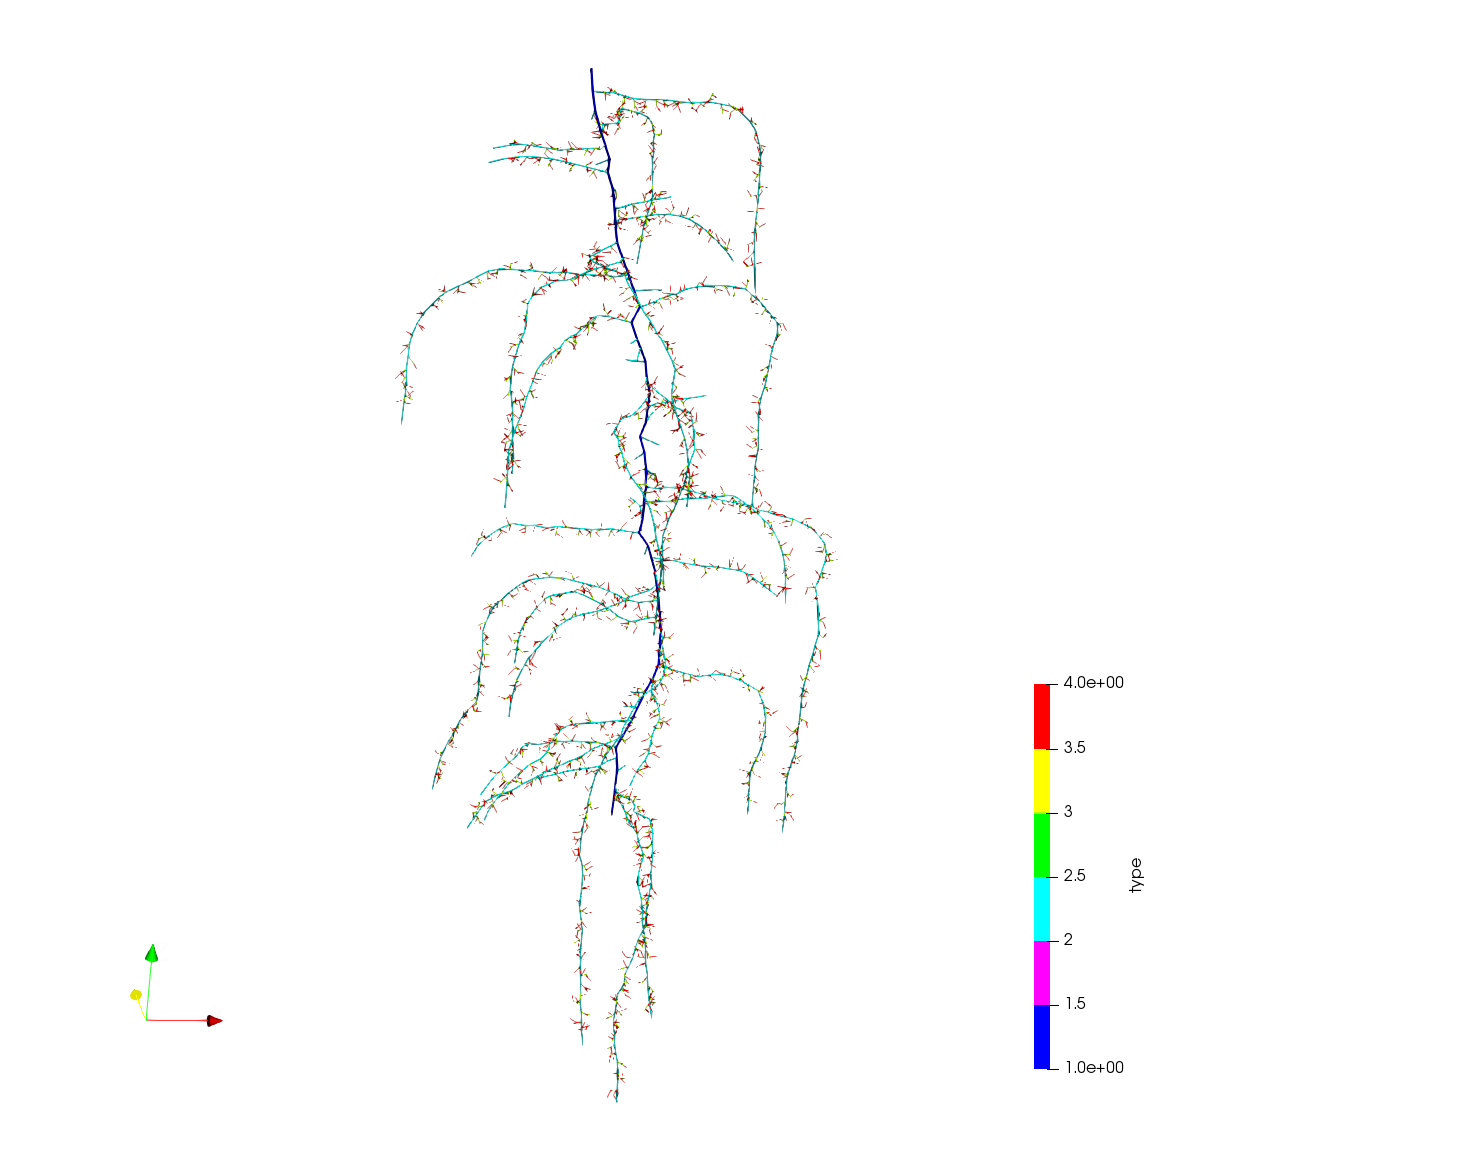
\includegraphics[width=0.7\textwidth]{example4b.png}
\caption{Depending on root age the laterals follow plagio- or gravitropism (Example 4b)} \label{fig:tropism}
\end{figure}



\newpage
\section{Root functional modelling} \label{sec:functional}

Root growth is strongly influenced by pedo-climatic conditions, and plant internal state. CPlantBox offers 'build in' ways to develop such models , see \cite{schnepf2018crootbox}. 

CPlantBox is a bottom up model were root growth is first defined under perfect conditions. Adding mechanisms to take environmental conditions into account will alter the root system development by impeding root growth, and by changing soil allocation by roots due to root tropism and due to altered branching patterns.

In this section we assume static soil conditions, and demonstrate the predefined ways how the soil can affect root growth.
Dynamic soil conditions are described in the following section 'Model coupling'. 

Implemented root responses are the change in direction of the growing root tip, as described in Section \ref{sec:tropism}.
Further root responses are 
\begin{itemize}
 \item scaling of the elongation rate 
 \item change of insertion angle
 \item change of lateral emergence probability
\end{itemize}

\subsection{Scaling the elongation rate} \label{sec:elongation}

Root elongation rate is influenced by water content, temperature, soil density, solutes, and many more. Regarding the processes that are investigated, various models can be applied. In CPlantBox the elongation rate is scaled with no predefined interpretation, i.e. we have to define a elongation rate scaling, which is dependent on such soil properties. The following example defines two compartments (one left, one right), where we change the scaling, and can analyse the results. The same procedure will be used in Example \ref{sec:insertion_angle} and \ref{sec:branching}.

\lstinputlisting[firstline=1, language=Python, caption=Example 5a]{../../examples/python/example5a_elongation.py}

\begin{itemize}

\item[7-10] Creates the root system and opens the parameter file.

\item[13-17] We create a confining box with two overlapping boxes called left and right. These geometries are used for later analysis.

\item[20-24] We define static soil properties using SDF (L23, L24) as we did in Section \ref{sec:hydro}. 
The left compartment has the value $minS$, the right $maxS$, between them is a linear gradient of length $slope$.

\item[27-31] Sets the scaling functions. L29 adjusts axial resolution and L30 tortuosity $sigma$. L31 sets the scale elongation function $f_{se}$ to the soil property (i.e. scales to $minS$ in the left, $maxS$ in the right compartment). 

\item[34-39] Initialization and simulation loop. In a dynamic setting, $soilprop$ needs to be updated in each time step (comment L38).

\item[42-50] Analysis the root length in the left and right compartment. With parameters $minS$ and $slope$ only $21\%$ are located in the left compartment.

\item[53, 54] Writes the results for Paraview visualization (see Figure \ref{fig:elongation}).

\item[57] A vtk simulation of root lengths. Press 'y' to obtain a x-z view of the root system to better see the effect. 

\end{itemize}
 
Next, we give a short layout, how the code would look like, if we take measured data (e.g. density versus depth), and include it in the simulation. 

\lstinputlisting[firstline=1, language=Python, caption=Example 5b]{../../examples/python/example5b_scaleelongation.py}

\begin{itemize}

\item[12-18] In L12 an EquidistantGrid1D is created, which is a specialisation from SoilLookUp (in soil.hh). It represents a 1D grid from 0 cm to -100 cm as soil with 100 layers. Additionally scalar data are attached to the grid, L13, L14 we create example soil strength data. From this data we calculate the elongation scales (L15), and set it as grid data (L16). 

\item[L17, L18] Retrieve the elongation scale data at two points. The data is given per layer, no data interpolation is performed.

\item[20, 21] Sets the elongation scaling function to all root types.

\item[25-32] Subsection \ref{ssec:animation} explains how to make an animation in Paraview. Here we use another (slower) approach to create the animation (and a preview) directly in vtk. For this we create an AnimateRoots object (L26), choose the domain size, and start the rendering (L32). 

\item[34-50] Simulation loop. If soil strength changes, the elongation scales must be calculated again (L32), and attached to the grid (L35). The frames of the animations are written in L50. While the approach is convenient, it is rather slow since for each frame a SegmentAnalyser object is created and rendered from scratch which is not feasible for large root systems. 

\item[39,40] Exports results as vtp, and creates a vtk plot. The effect of the dense layer can hardy be seen in the results (between -10 and -15 cm depth, laterals will be shorter). But the created animation reveal the effect (see exported video example5b.ogv). 

\end{itemize}

\begin{figure}
\begin{subfigure}[c]{0.32\textwidth}
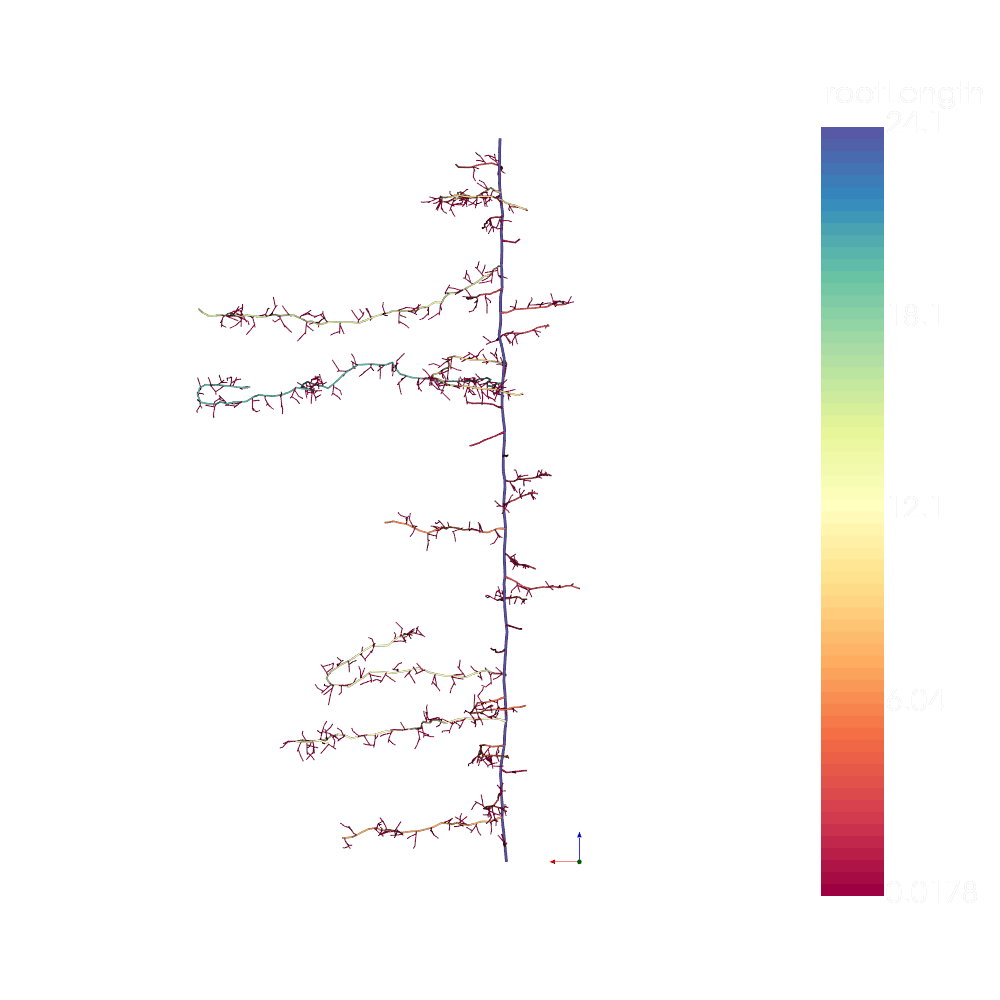
\includegraphics[width=0.99\textwidth]{example5a.png}
\subcaption{Root elongation rate} \label{fig:elongation}
\end{subfigure}
\begin{subfigure}[c]{0.32\textwidth} 
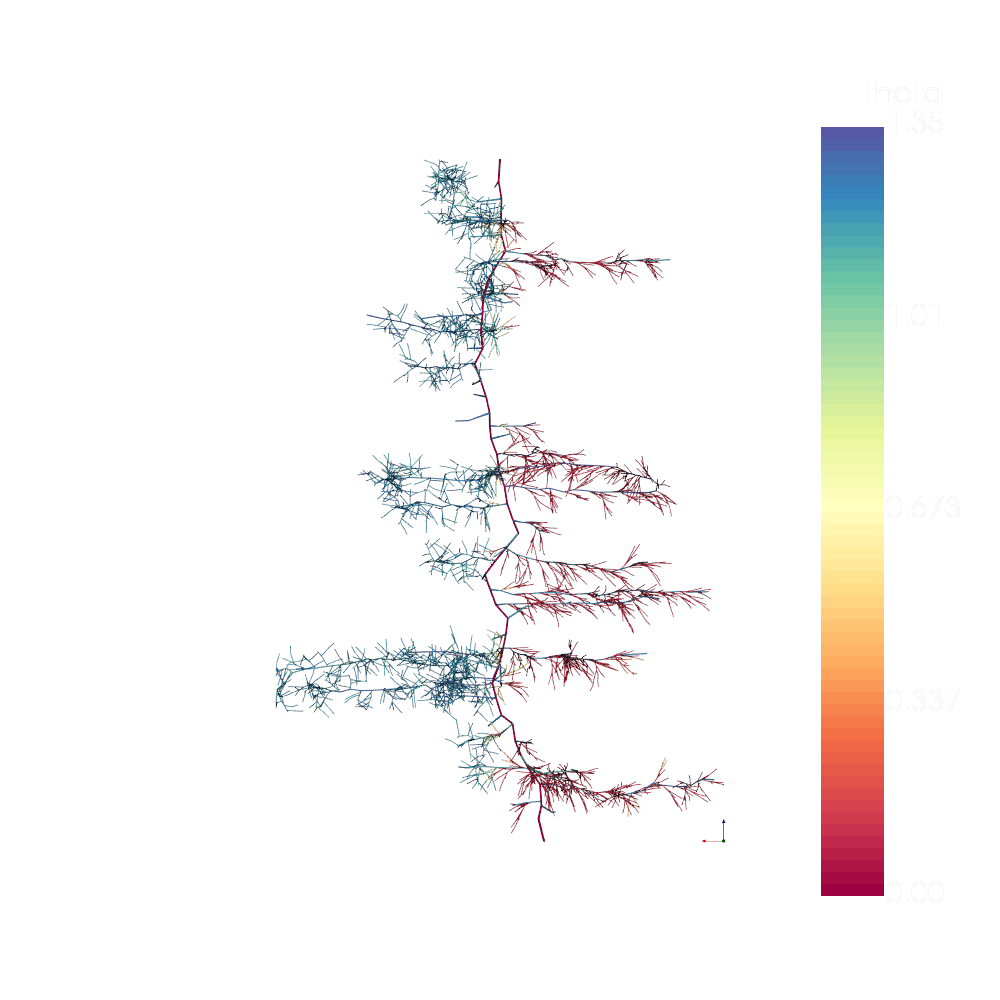
\includegraphics[width=0.99\textwidth]{example5c.png}
\subcaption{Insertion angle} \label{fig:insertion}
\end{subfigure}
\begin{subfigure}[c]{0.32\textwidth}
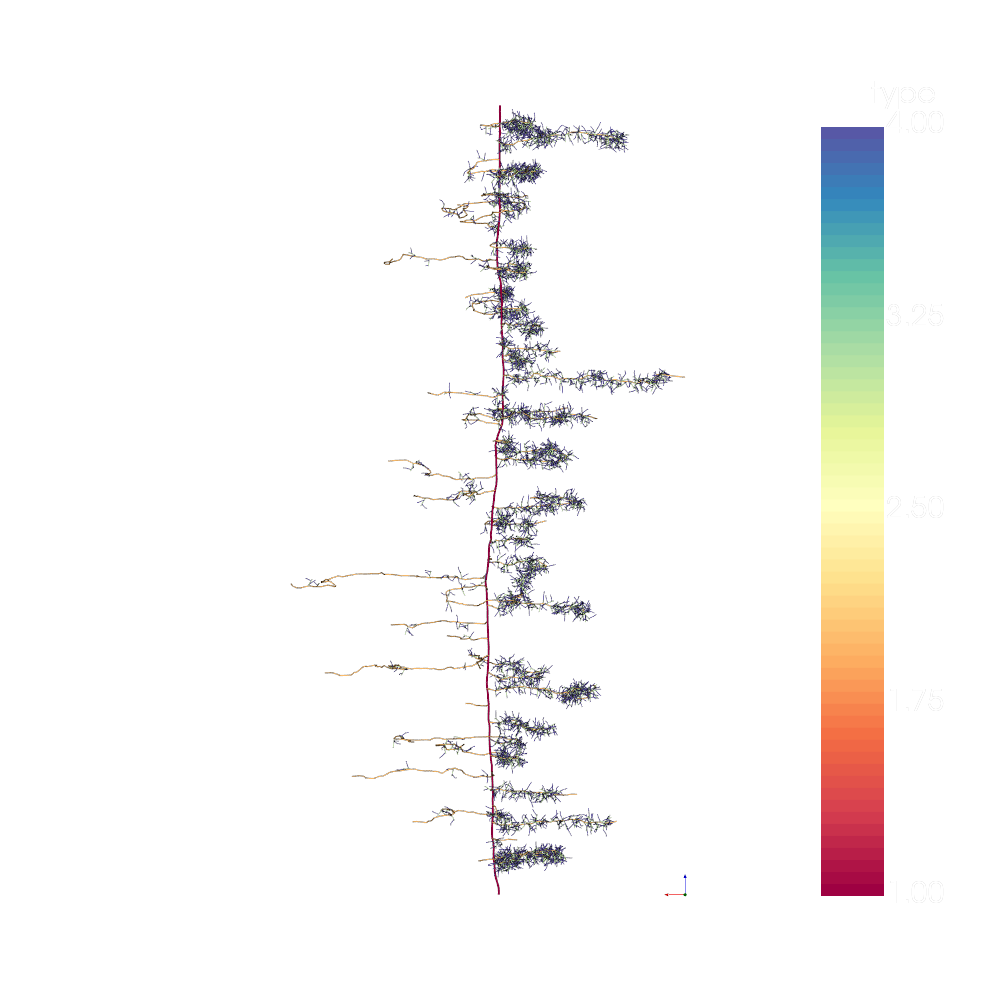
\includegraphics[width=0.99\textwidth]{example5d.png}
\subcaption{Branching density (probabilistic model)} \label{fig:probability}
\end{subfigure}
\caption{Predefined root responses (Example 5a)}
\end{figure}



\subsection{Change of insertion angle} \label{sec:insertion_angle}

Nutrient concentration can influence the angle between parent roots and laterals (ref what else).

Analog to Example 5a two compartments are created, and the insertion angle is scale altered accordingly.

\lstinputlisting[firstline=1, language=Python, caption=Example 5c]{../../examples/python/example5c_insertionangle.py}

\begin{itemize}

\item[7-10] (as before) Creates the root system and opens the parameter file.

\item[13-17](as before) We create a confining box with two overlapping boxes called left and right. These geometries are used for later analysis.

\item[20-24] (as before) We define a static soil properties using SDF (L23, L24) as we did in Section \ref{sec:hydro}. 
The left compartment has the value $minS$, the right $maxS$, between them is a linear gradient of length $slope$.

\item[27-32] Sets the insertion angle scaling functions to second order laterals only (L29). L20 adjusts axial resolution and, L31 tortuosity $sigma$, and L32 sets the scale insertion angle function $f_{sa}$ to the soil property. Additionally, the maximal length of second order roots is redoubled. 

\item[34-39] Initialization and simulation loop.

\item[42-50] Analysis the root insertion angle in the left and right compartment. 

\item[53, 54] Writes the results for Paraview visualization.

\item[57] A vtk simulation of root lengths. Press 'y' to obtain a x-z view of the root system to better see the effect (see Figure \ref{fig:insertion}). 

\end{itemize}




\subsection{Change of lateral emergence probability} \label{sec:branching}

Soil properies can affect branching patterns. In the following example analog to Example 5a two compartments are created, and the branching probability is modified.

\lstinputlisting[firstline=1, language=Python, caption=Example 5d]{../../examples/python/example5d_branching.py}


\begin{itemize}


\item[27-30] Adjusts axial resolution and tortuosity.

\item[33, 34] We adjust the inter lateral distances by making it smaller for a factor five.

\item[35, 36] We set the branching probability scaling for the second order laterals. The scaling value means the probability that the branch occurs per day, i.e. 1 means the laterals alwas emerge (left compartment), or that they emerge with a chance of 0.2 \% per day (right compartment). 

\item[46-54] Analysis the root insertion angle in the left and right compartment. 

\item[63] A vtk simulation of root lengths. Press 'y' to obtain a x-z view of the root system to better see the effect (see Figure \ref{fig:probability}). 

\end{itemize}

Note that a scaling of 0 means, that the lateral does never emerge, 1 means they always do. While the branching is very limited, it is easy to modify it to implement plant systemic responses. For this a suitable SoilLookUP must be defined and the method getValue(x, organ) must be overwritten, implementing the plant control of the branching probabilities. 




\newpage
\section{Coupling to numerical models} \label{s:coupling}

CPlantBox is a bottom up model where no water movement or solute transport is calculated per default. The idea is to make it easy to link the root growth model to any numerical models or solvers. This is achieved by member functions that make it easy to (a) obtain a numerical grid from the root system, and (b) to offer utility functions to map root segments to an underlying soil grid. 

In this section we consider a static root system. The additional steps that are needed for a developing root system (i.e. with a changing root geometry) are explained in the next section. 

\subsection{Mapping between root segments and an underlying soil} \label{ss:mapping}

The classes MappedSegments and MappedRootSystem, defined in MappedOrganism.h, manage the coupling between the root system and external models or solvers. 

The RootSystem class stores the nodes of each root in an object of class Root. This is convenient for simulating the root development, but not suitable for coupling to numerical models. Commonly, numerical models need the nodes as sequential list (obtained by RootSystem::getNodes) and the information on how they are connected (e.g. RootSystem::getSegments). Additionally, some information on the segments like radius or root type is needed. Furthermore, when coupling to a soil model, we need information in which soil cell the segment is located, and vice versa, which segments are located within a specific soil cell. 

The class MappedSegments helps to manage all that, and offers the data structure for sequential nodes, connections between two nodes as segments, and the most commonly needed data such as creation time of the node, and radius or type per segment. Most important, it contains two hash maps seg2cell and cell2seg, linking segments to cells, and cells to list of segments.

MappedRootSystem is derived from MappedSegments and RootSystem, i.e. it can be used in the exact same way as the RootSystem class, but keeps track of the lists, and (optionally) the mapping between soil grid and root system.

To demonstrate basic functionality we will map a root system to a soil rectangular soil grid. 

\lstinputlisting[firstline=1, language=Python, caption=Example 6a]{../examples/example6a_mapping.py}

\begin{itemize}

\item[8-12] Creation of a small root system. Instead of the class RootSystem, MappedRootSystem is used (L8). MappedRootSystem is a specialisation of the 'normal' RootSystem class and can be used in the exactly same way. 

\item[16-19] We choose a small soil domain, where some roots are not inside. Calling MappedRootSystem::setRectangularGrid first cuts segments at the cell faces, and then maps the resulting segments to a soil index (creates the maps MappedRootSystem::seg2cell, and MappedRootSystem::cell2seg). The value True indicates that cutting is performed, False just maps the segment mid points without cutting. 

\item[22-28] Next we create an array $x$ containing the soil indices for each segment, that will be later used for vizualisation. We use the hash map (a Python dictionary) MappedRootSystem::seg2cell to obtain the linear index of the cell, where the segment's mid point is located.

\item[31-37] To demonstrate how to retrieve all segments that lie within a given cell, we output the segments at the cell located around the position [0,0,-7]. In L31 we retrieve the cell index for that position. L34 and L35 print out the segment indices. Note that the map will have no entry for a given cell, if no segments are located in the cell. 

\item[43-48] To visualize the soil cell indices, we first create a SegmentAnalyser class. The class MappedRootSystem is derived from a RootSystem and MappedSegments. If we create a SegmentAnalyser class directly from $rs$ (L40) MappedRootSystem will be considered as RootSystem, and the resulting class will contain the original segments before cutting at the cell boundaries. The function MappedRootSystem::mappedSegments (L41) will return a reference to $rs$ but with the type MappedSegments. In this way the SegmentAnalyser class will be created including the cut segments. Next, in L42 we add the indices as data to the SegmentAnalyser class. L43, L44 produces the VTK plot, but rendering is started at a later point, since we also want to visualize the underlying soil grid.

\item[51-53]  L47 creates the mesh for vizualisation, L48 creates the VTK plot, and L49 starts the rendering window, rendering both, root system and underlying soil. Press 'y', 'x', and 'z' to obtain axis aligned views of the root system and soil grid.

\end{itemize}

More, generally, when coupling to an external solver like DuMux \citep{koch2020dumux}, we need to set the soil$\_$index function, that returns the cell index for a certain position. Additionally, periodic soil domains are already implemented. Both coupling to DuMux and periodicity will be demonstrated in Section \ref{sec:dumux_coupling}.

Coupling to an unstructured grid is as simple as to a structured one. But automatic cutting of segments at the cell faces is currently not implemented. That means that axial resolution should be small in order to keep the introduced error small.



\subsection{Water movement within the roots} \label{ssec:xylem}

Since water movement within the roots is often needed, it is implemented directly in CPlantBox (in the class XylemFlux) following \cite{meunier2017hybrid}. However, usage is optional, and any other transport code can be used (e.g. if solutes are considered). XylemFlux sets up the linear system, and the sparse linear system is then solved in Python using scipy (using the class XylemFluxPython defined in xylem$\_$flux.py).

The following example is based on benchmark M3.1 \citep{schnepf2019call} with constant conductivities, but not with a given root system, but a simulated one.

\lstinputlisting[firstline=1, language=Python, caption=Example 6b]{../examples/example6b_xylemflux.py}
\begin{itemize}

\item[11-15] All parameters that will be used later on.

\item[18-23] The root system (similar to last section). 

\item[26-31] The MappedRootSystem is wrapped with the XylemFluxPython class, which extends the XylemFlux class, which computes the xylem matric flux potential. L27, L28 sets the radial and axial conductivity. L29 retrieves the root system nodes for later visualisation. The pressure surrounding the the root system is either defined as pressure surrounding each root segment, or as soil cells, in which the root segments are located. L30, L31 sets a soil containing of one single cell with index 0. 

\item[34-36] XylemFluxPython defines solvers like solve$\_$dirichlet for Dirichlet boundary condition (predefined collar matric potential), solve$\_$neumann for Neumann boundary condition (predefined collar flux), and solve which switches between Dirichlet and Neumann at some critical pressure (the plant wilting point).
The arguments of solve$\_$dirichlet are the simulation time (to calculate age dependent conductivities), the root collar pressure head, the pressure around the root collar, the soil matric potential around the root segments or per soil cell, and a boolean value that decides if the potentials are given per soil cell (True) or per segments (False). The return value $rx$ contains the xylem matric potentials per segment. L35 calculates the fluxes into the soil (negative values mean into the root). The bool argument determines if we approximate the flux, or use the exact solution by \cite{meunier2017hybrid}.
L36 determines the root collar flux.

\item[39-43] Plots the results.

\item[46-49] Creates the VTK plot, adding the soil matric potentials and fluxes. L49 picks either $rx$ or $fluxes$ for vizualisation, see Figure \ref{fig:xylemfluxa} and \ref{fig:xylemfluxb}.

\end{itemize}

It is possible to set conductivties per root type (see XylemFlux::setKr, and setKx), and root age dependent conductivities per root type using linear lookup tables (see XylemFlux::setKrTables, and setKxTables).

\begin{figure}
\begin{subfigure}[c]{0.5\textwidth}
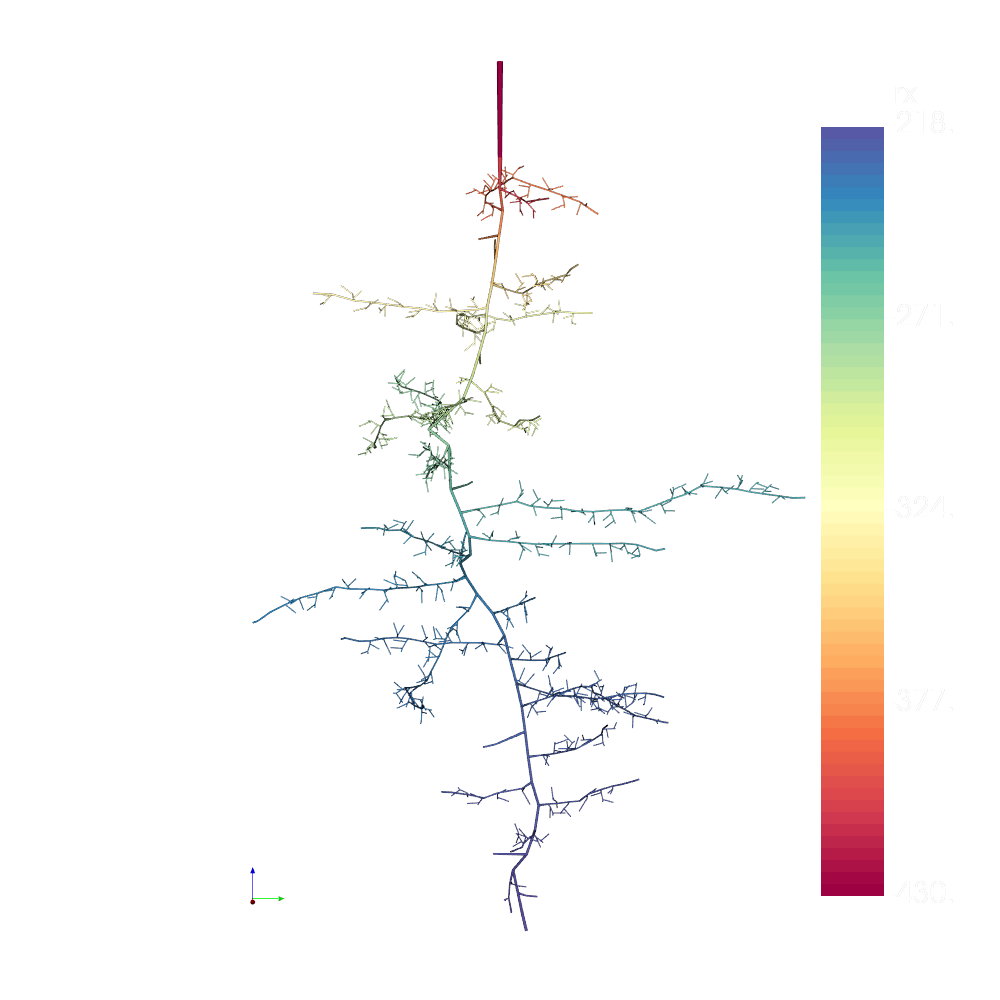
\includegraphics[width=0.99\textwidth]{example6b.png}
\subcaption{Anagallis} \label{fig:xylemfluxa}
\end{subfigure}
\begin{subfigure}[c]{0.5\textwidth}
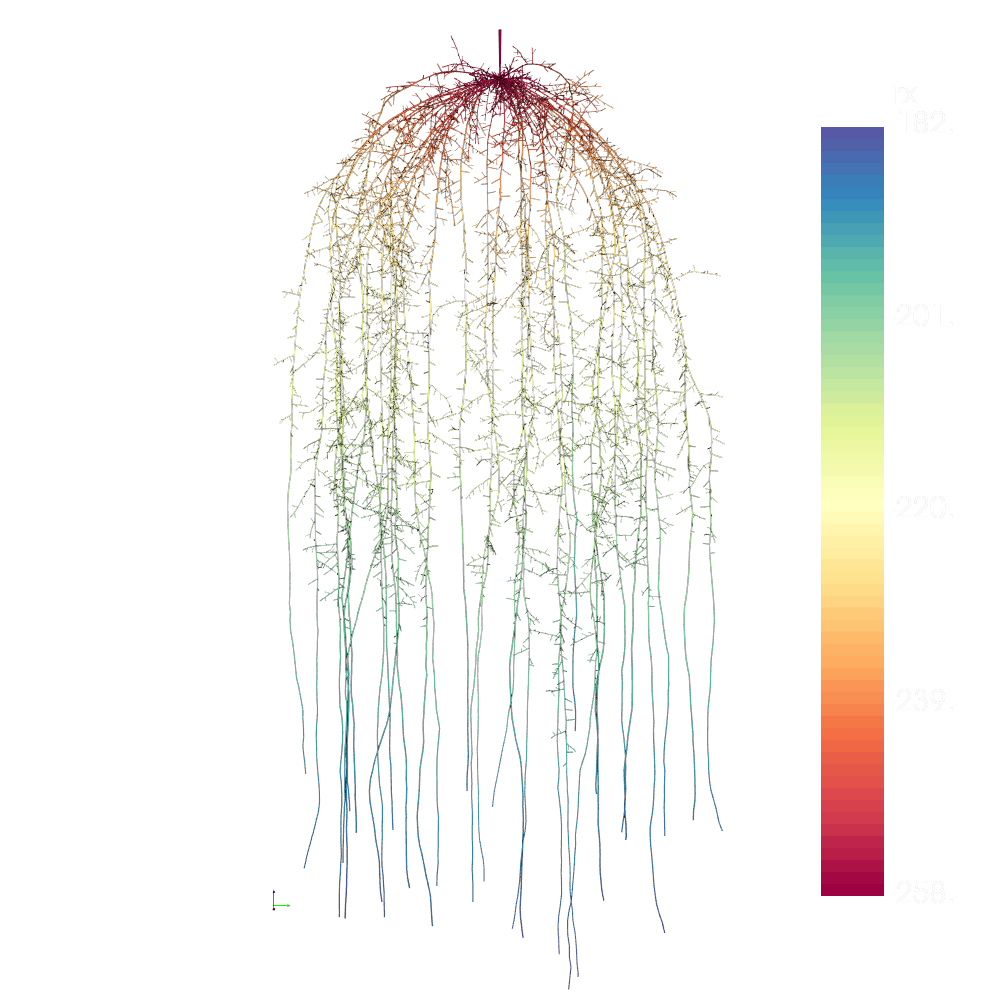
\includegraphics[width=0.99\textwidth]{example6b_2.png}
\subcaption{Maize} \label{fig:xylemfluxb}
\end{subfigure}
\caption{Calculated xylem matric potential (cm)} 
\end{figure}

\subsection{Stomatal modul} \label{ssec:stomatal}

The following example presents the stomatal modul (see file example6e$\_$xylemflux$\_$variable$\_$gs.py). The actual evapotranspiration (ETa) of the plant is determined according to environmental parameters, root and leaf surface, and maximal stomatal conductance (gmax). 
%\lstinputlisting[firstline=1, language=Python, caption=Example 6e]{../examples/example6e_xylemflux_variable_gs.py}
\begin{itemize}

\item[11-19] Part of the parameters that will be used later on.

\item[18-23] The root system (similar to last section). 

\item[21-25] Creation of the plant object, definition of the grid and simulation of the plant growth.

\item[38-42] Set the parameters for the calculation of the actual leaves radial conductivity (gs) and ETa using the equations of [TOADD].

\item[44-48] Get the plant nodes and tips to set the Neumann boundary conditions (i.e. 0 axial flux is set at the plant nod tips (i.e: water only enters/leaves the plant by radial flux)

\item[51] Solve the water flux using the Neumann boundary conditions. The program then loops on the calculation of ETa, xylem potential, and gs until convergence or after having done 1000 loops. p$\_$linit and gmax are respectively the initial leaf xylem potential and initial leaf radial conductivity used in the loop.

\item[52] Calculation of the radial fluxes of each plant segment.

\item[53] Gives an overview of the water fluxes in the plant. If show$\_$matrices = True, the matrices with the axial and radial water fluxes for each plant segment is shown.

\item[62-72] Plots the results (see Figure \ref{fig:stomata} and \ref{fig:stomatb}).

\item[75-78] Creates the VTP file, which can then be opened in Paraview.

\end{itemize}

\begin{figure}
\begin{subfigure}[c]{0.5\textwidth}
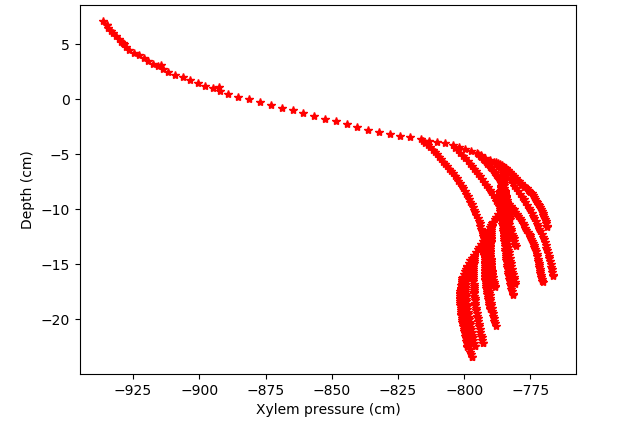
\includegraphics[width=0.99\textwidth]{example6e.png}
\subcaption{Calculated xylem matric potential (cm)} \label{fig:stomata}
\end{subfigure}
\begin{subfigure}[c]{0.5\textwidth}
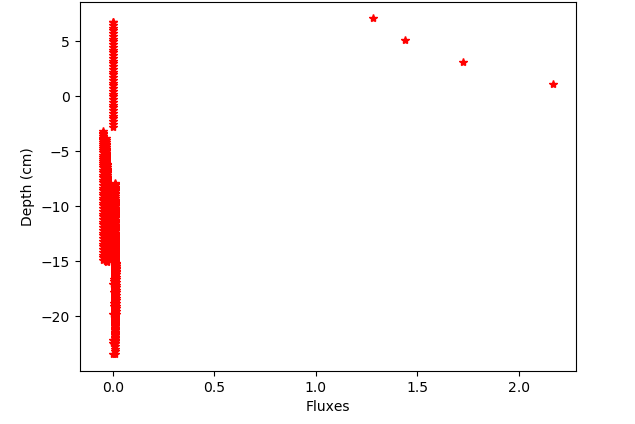
\includegraphics[width=0.99\textwidth]{example6e_2.png}
\subcaption{Radial water fluxes} \label{fig:stomatb}
\end{subfigure}
\caption{xylem potential and radial water fluxes per segment} 
\end{figure}

\subsection{Coupling a static root system to DuMux} \label{sec:dumux_coupling}

Putting the sections \ref{ss:mapping} and \ref{ssec:xylem} together, we can easily set up an example, using the classic sink term in the soil model, similar as in \citep{leitner2014impact} based on \citep{doussan1998modelling}. For solving the Richards equation we use DuMux \citep{koch2020dumux}.

The next example mimics benchmark C12 \citep{schnepf2019call}, but with a static simulated root system. The example must be run out of dumux-rosi (located in dumux-rosi/rosi$\_$benchmarking/python$\_$solver/coupled), otherwise the DuMux Python coupling is not available. 

\lstinputlisting[firstline=1, language=Python, caption=Example 6c]{../examples/example6c_coupling.py}

\begin{itemize}

\item[3,4] Add paths for DuMux Python coupling (L3) and Python solvers (L4).

\item[5,6] The direct C++ part of the DuMux binding, and the Python wrapper class. 

\item[17,18]  Defines a sinusoidal function for the collar boundary condition.

\item[21-37] All parameters that are needed for this simulation. L25 decides if periodic boundary conditions are used, or not. L35 states the simulation time, L36 the initial root system age. L37 defines if age dependent root conductivities are used. The rooot conductivities are hard coded in the file root\_conductivities.py, that is imported in L8. Age dependent conductities can be used to mimic root growth in a predefined way, i.e. the root system is already fully grown, but the radial conductivities are turned on during the simulation. 

\item[41-49] Sets up the soil solver (DuMux Python binding from dumux-rosi). 

\item[52-62] Sets up the Xylem model as in Subsection \ref{ssec:xylem}. If the root system is not periodic, a confining geometry is set L54-L58. L62 passes the axial and radial conductivities to the XylemFluxPython object (the function is defined in root\_conductivities.py).

\item[65-70] Coupling between the soil soil and root part is performed by setting the picking function that assigns a cell index to each spatial position L65, and L66. In L67 root segments are cut to the rectangular grid, and in L70 the cell index of the root collar is determined. 

\item[73-77] Initializes the simulation, initially the soil values are the same as the initial conditions (L75).

\item[79-94] First, we calculate the xylem matric potential $rx$ for a given soil matric potential $sx$ (L81) and save the actual collar flux for later analysis (L83). Next, we calculate teh sink (L85) and apply it to the soil model (L86). The soil model is simulated (L87) and the resulting matric potential $sx$ is updated (L88). The simulation takes some time (around 15 minutes), and L90-93 print debugging information and a progress bar. L94 increases the current simulation time. This is needed if age dependent conductivities are used. 

\item[99-111] L99 creates Figure \ref{fig:example6c} and, L102-111 plots uptake and cumulative uptake over time, see Figure \ref{fig:uptake}.

\end{itemize}

\begin{figure}
\begin{subfigure}[c]{0.5\textwidth}
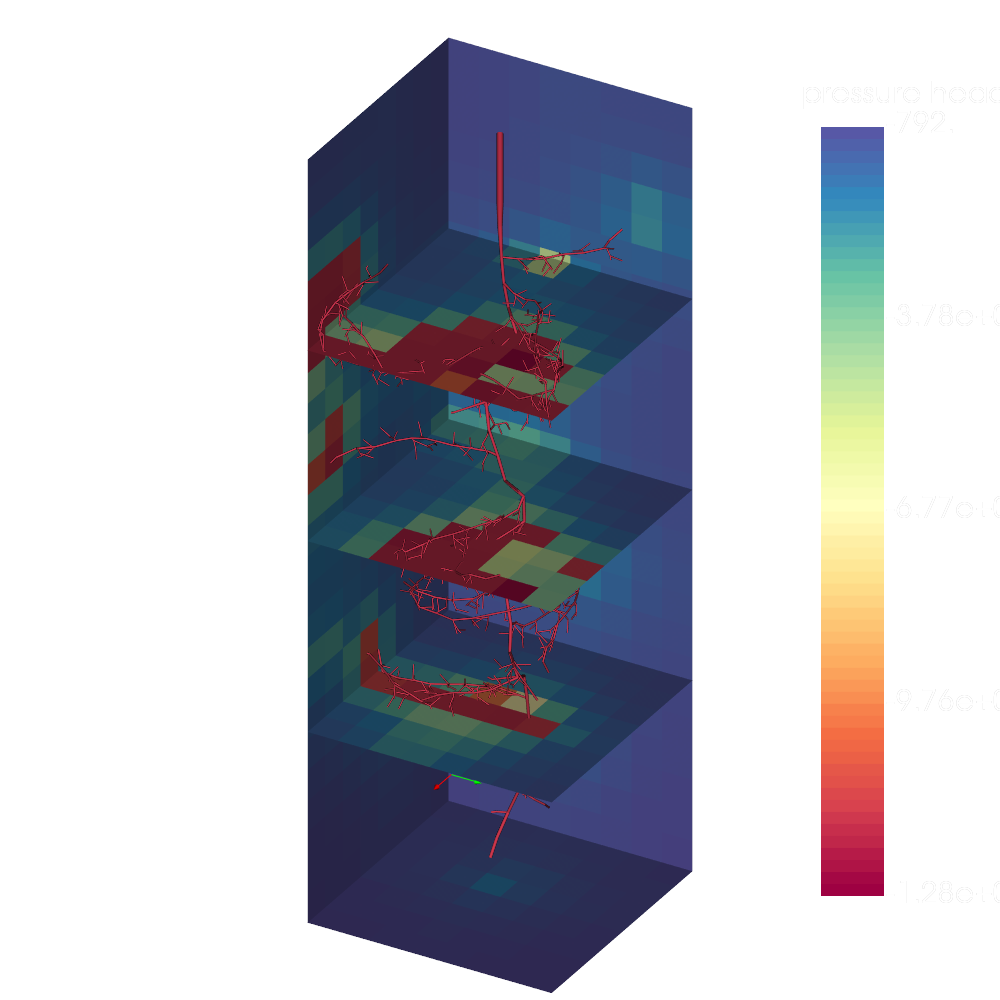
\includegraphics[width=0.99\textwidth]{example6c.png}
\subcaption{Confined} \label{fig:example6c}
\end{subfigure}
\begin{subfigure}[c]{0.5\textwidth}
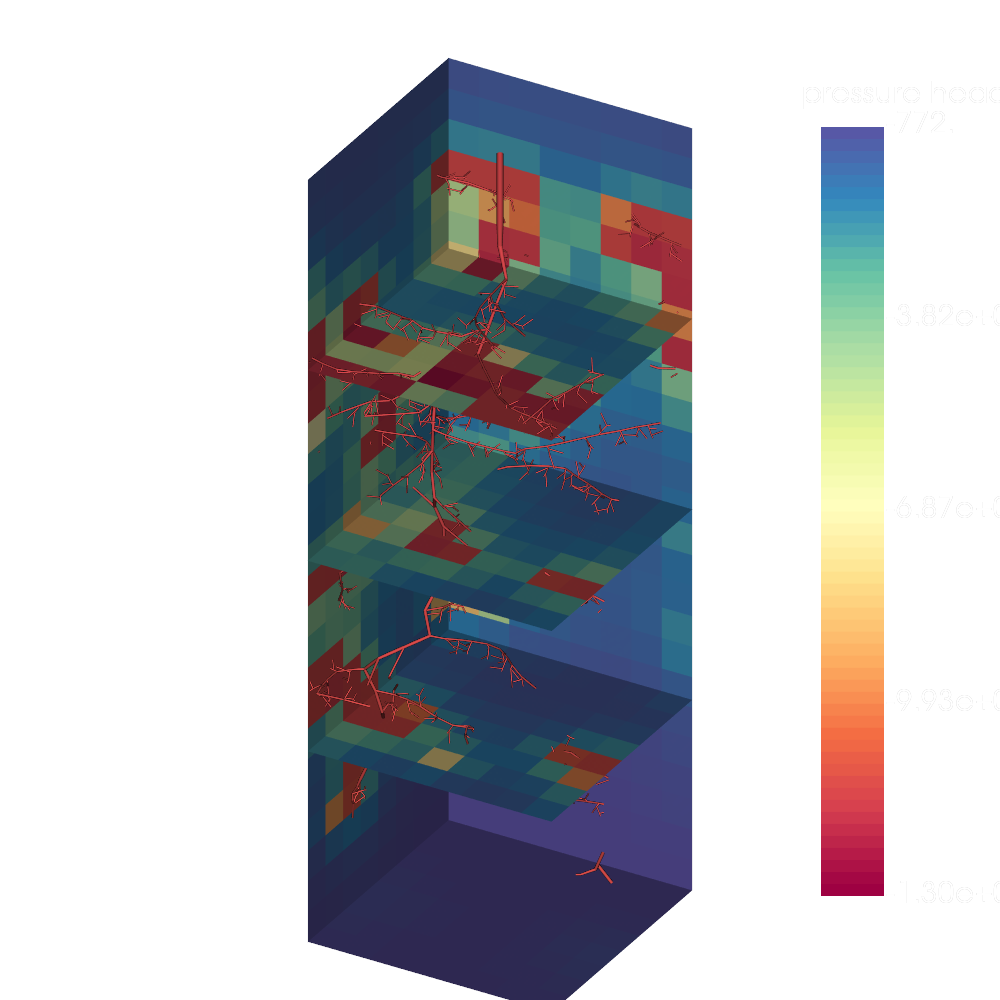
\includegraphics[width=0.99\textwidth]{example6c_periodic.png}
\subcaption{Periodic boundary condtions} \label{fig:example6c_peridodic}
\end{subfigure}
\caption{Water depletion due to root uptake after one week. } \label{fig:example6c}
\end{figure}

With above code we can compare total root system water uptake in a container, with the uptake if periodic boundary conditions are used. While the first scenario reflects the situation in a plant pot, periodic boundary conditions reflect the situation when the plant grows in the field, where the planting distance is approximately the domain size. Figure \ref{fig:uptake} shows both situations, showing that the boundary conditions will strongly affect total water uptake, because roots are less evenly distributed in the pot scenario and water redistribution is impeded by the pot boundaries.

\begin{figure}
\begin{subfigure}[c]{1\textwidth} 
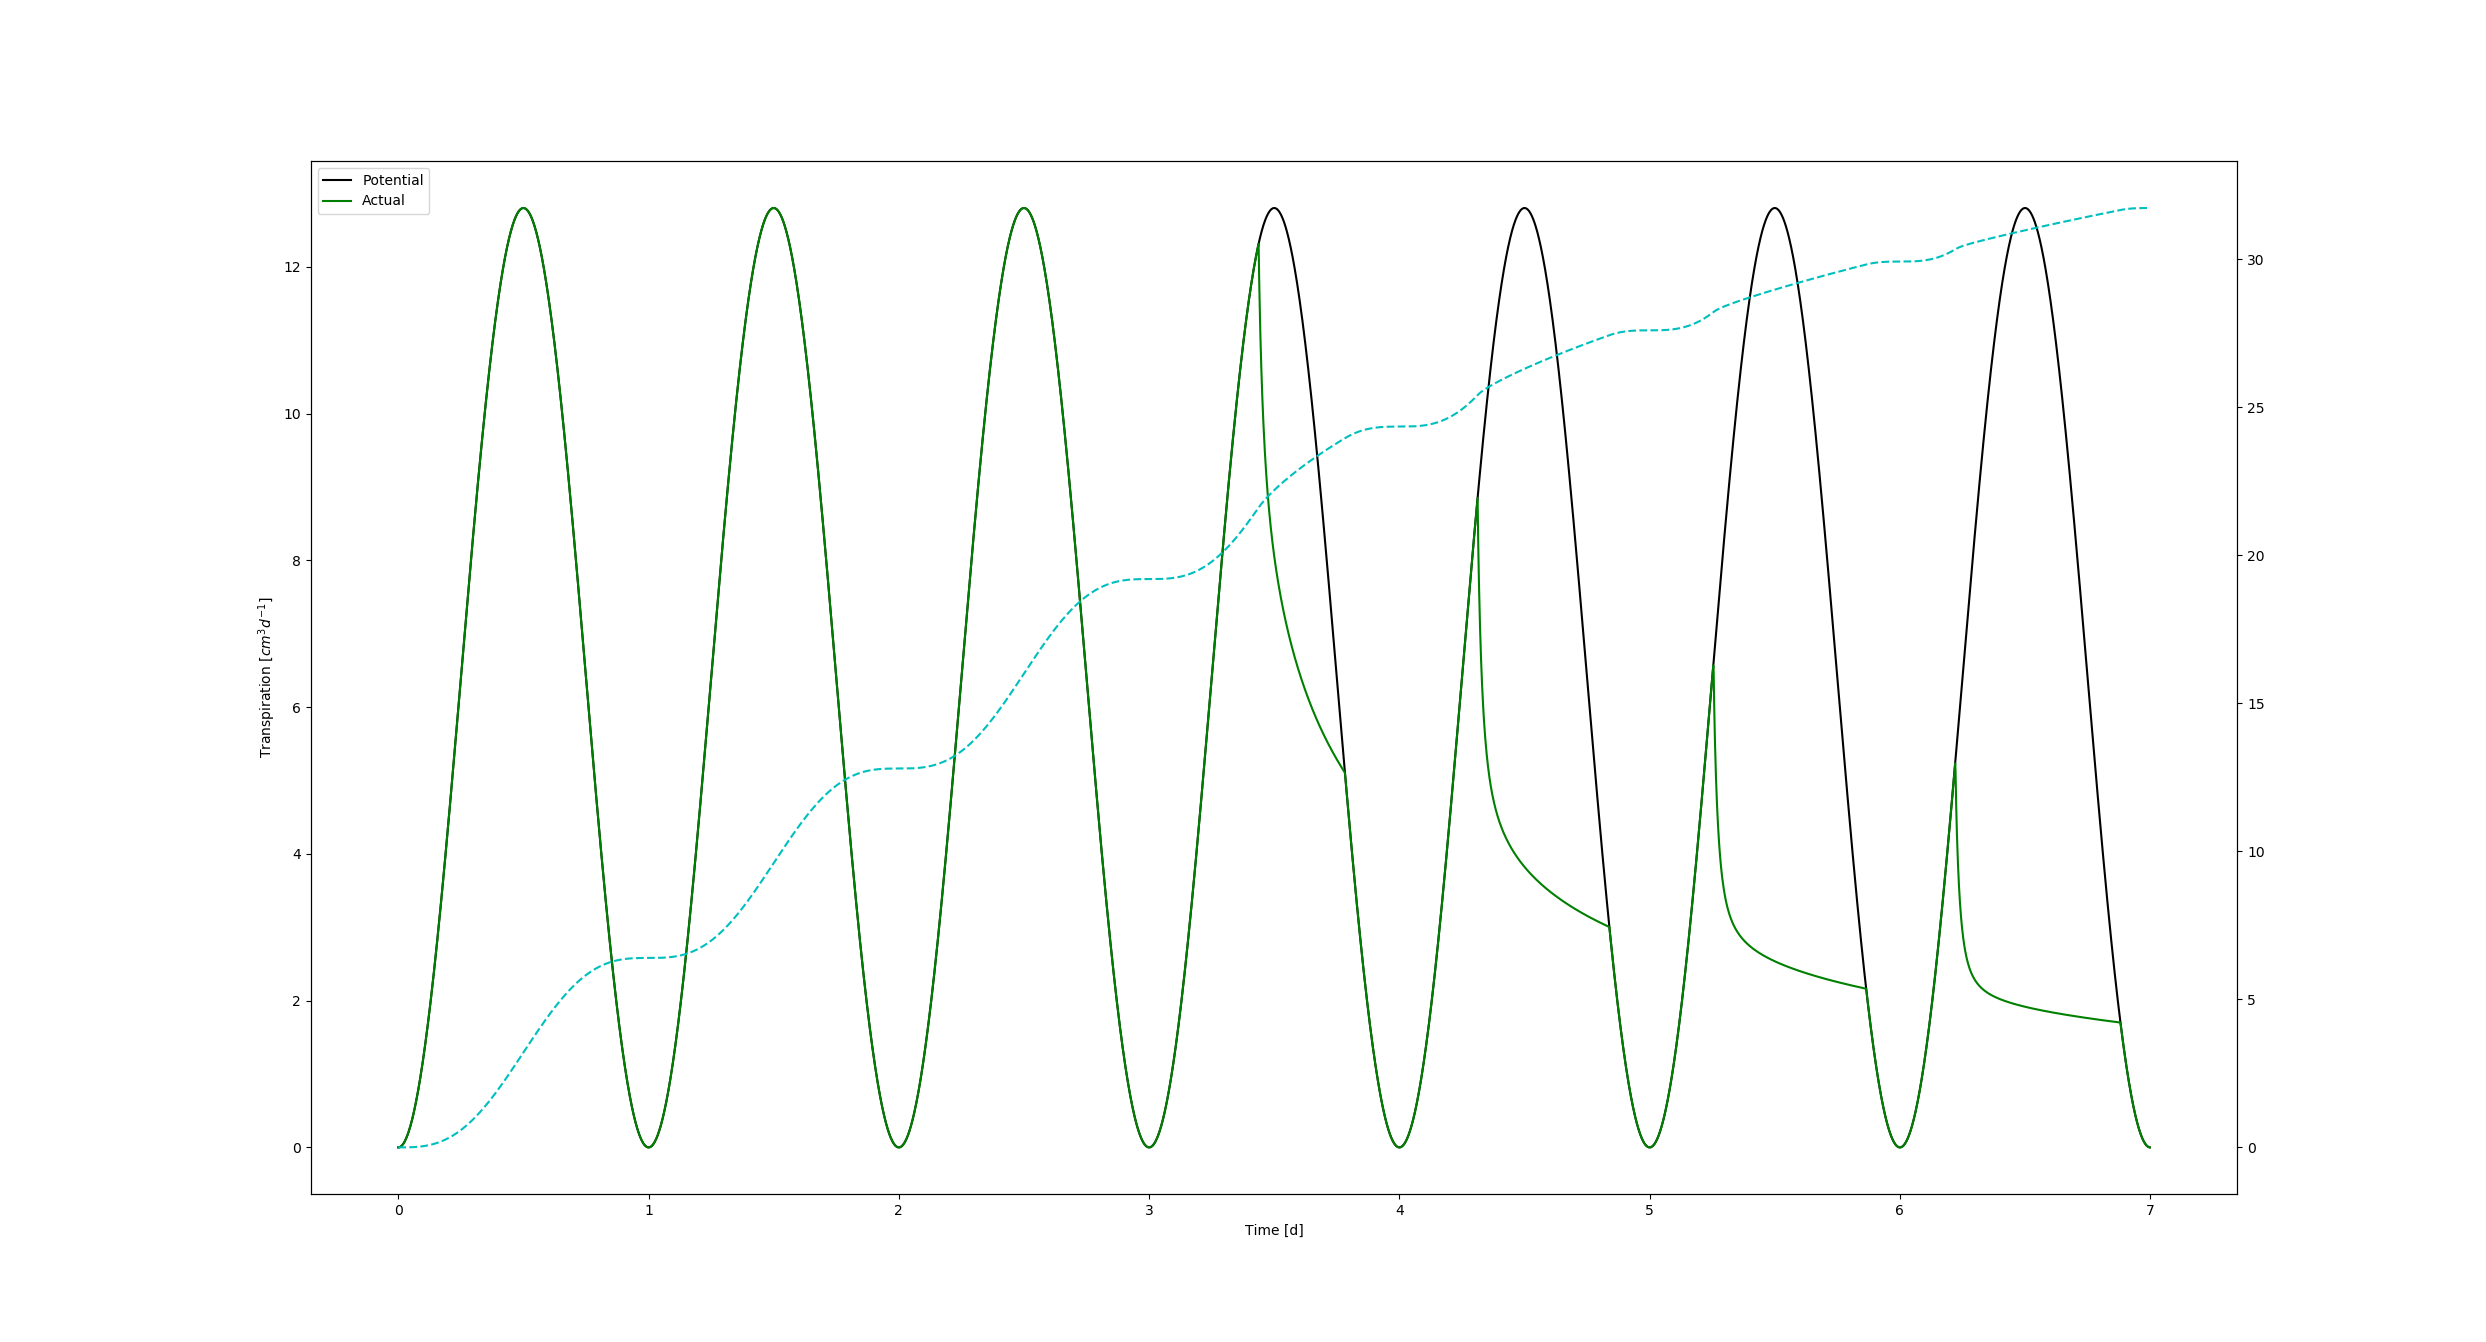
\includegraphics[width=0.99\textwidth]{Figure6c.png}
\subcaption{Confined} \label{fig:uptake_confined}
\end{subfigure}
\begin{subfigure}[c]{1\textwidth}
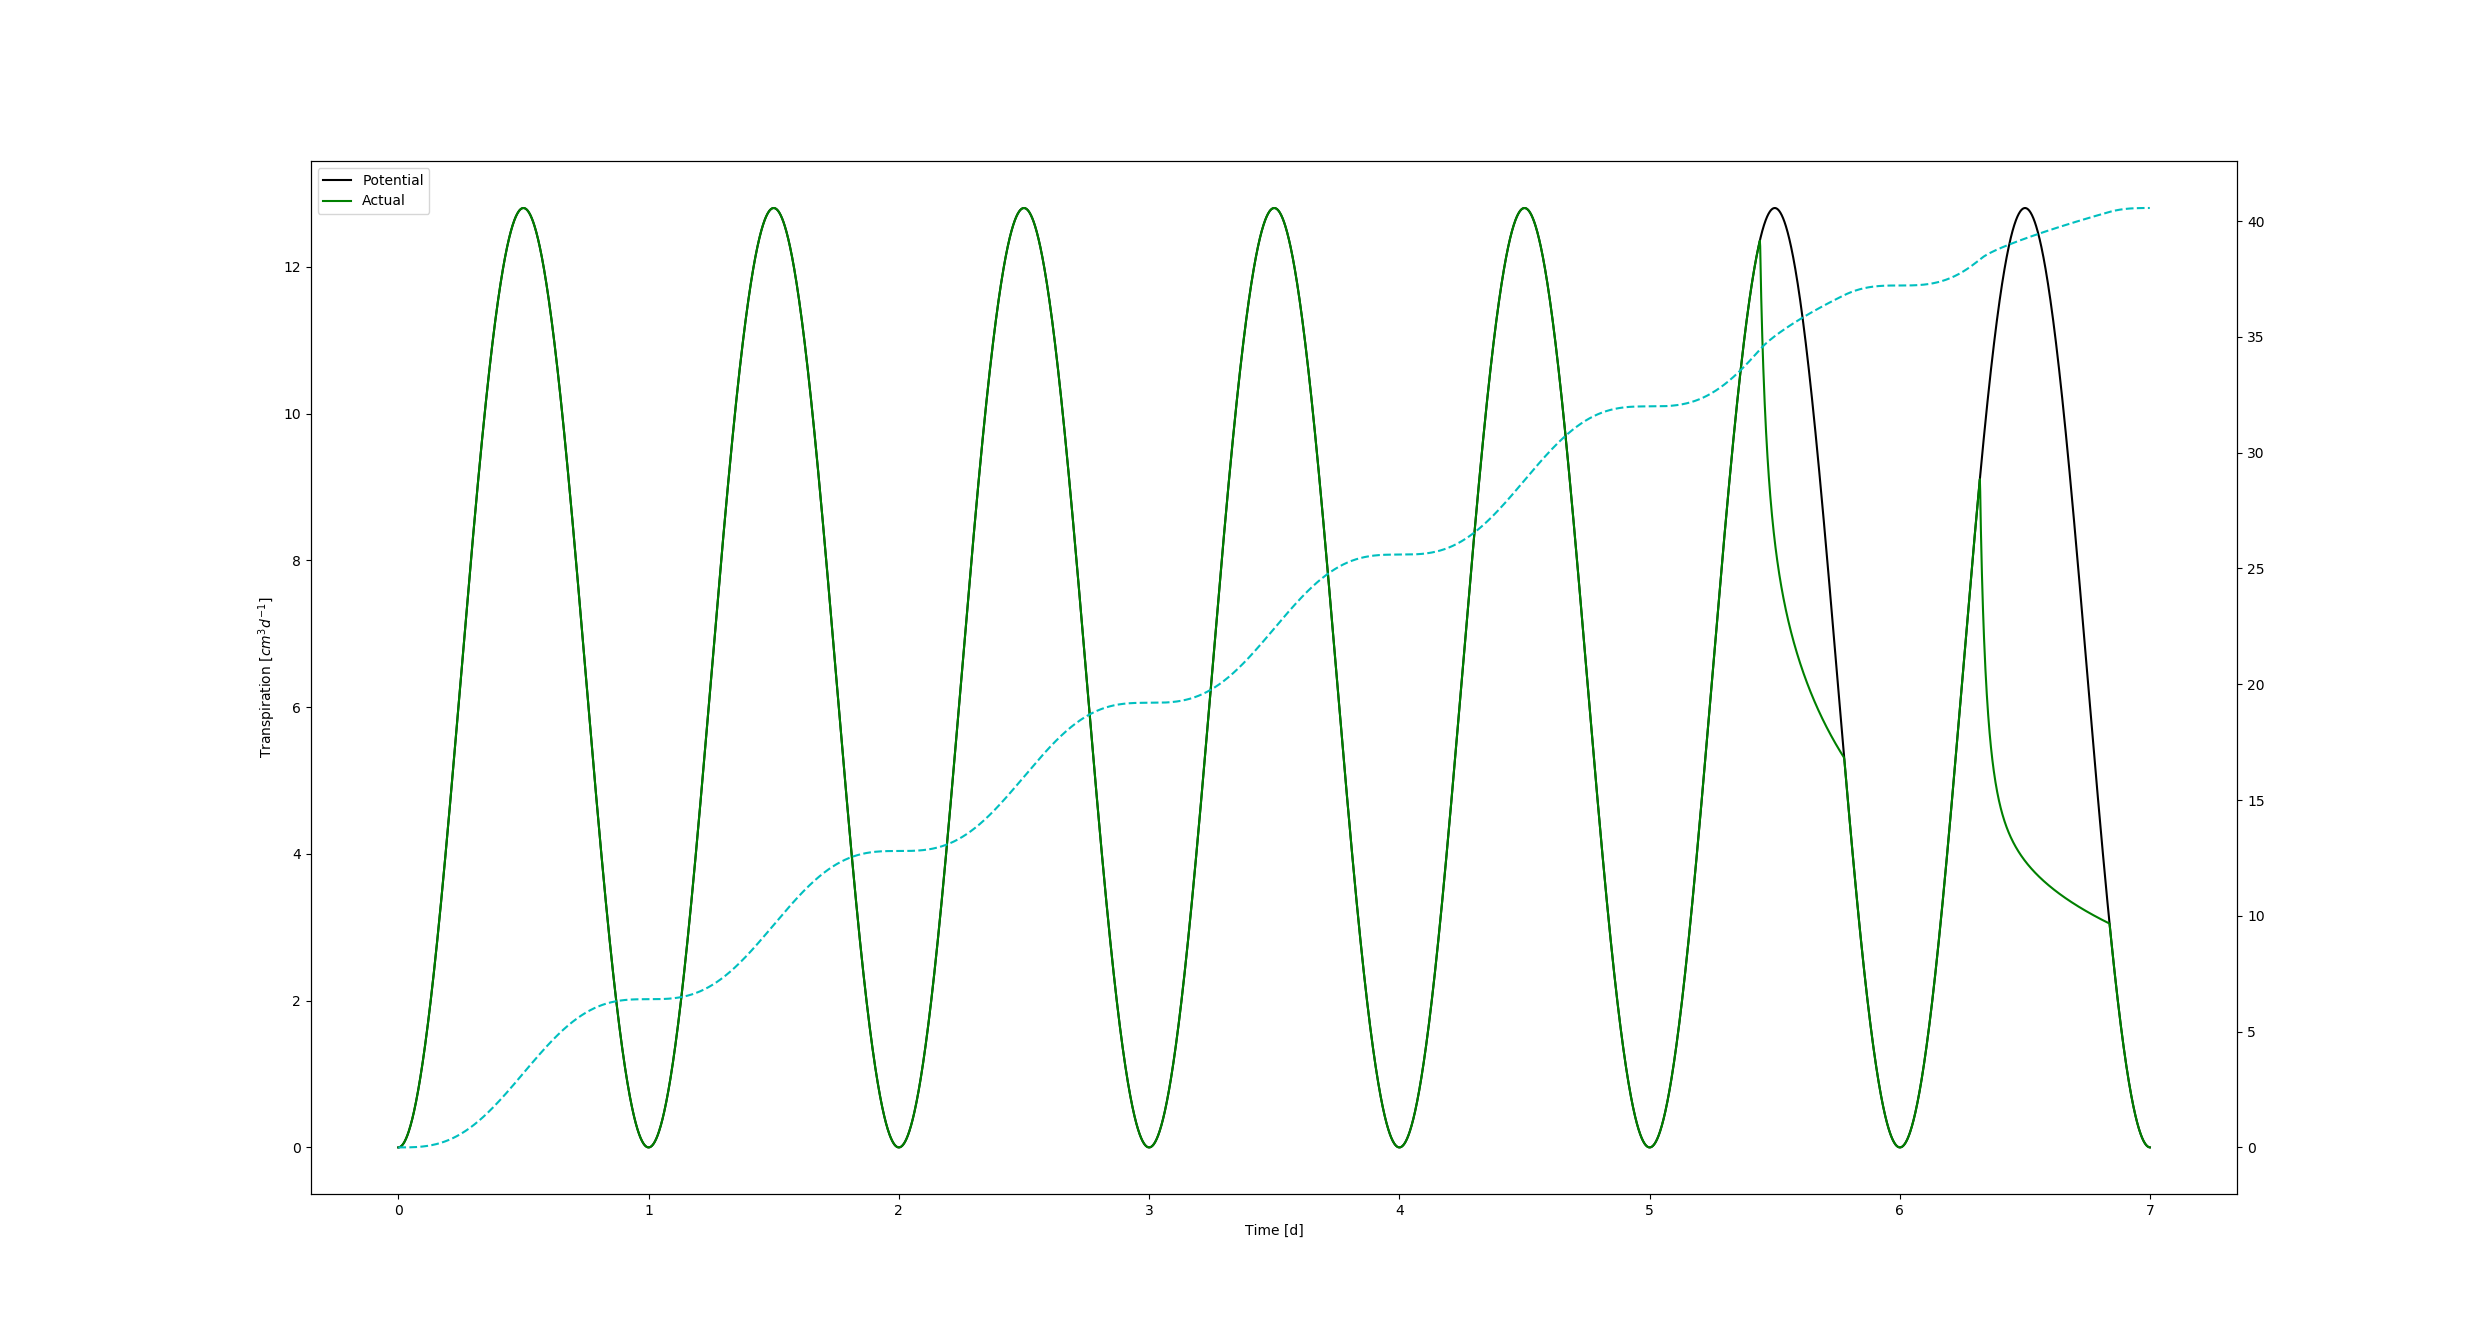
\includegraphics[width=0.99\textwidth]{Figure6c_periodic.png}
\subcaption{Periodic boundary condtions} \label{fig:uptake_peridodic}
\end{subfigure}
\caption{Water uptake and cumulated uptake} \label{fig:uptake}
\end{figure}





\newpage
\section{Coupling growing rootsystems to numerical models} \label{sec:growing}


In this section it is described how information about the last time step can be retrieved, 
and how we can incrementally obtain the root system from only new nodes and segments. 
These methods are especially important if we couple to other numerical software like DuMux


In the previous section root responses were described in a static soil. 
In this section we will extend this to a dynamic soil setting, where we update the soil in the simulation loop, and then update the root system iteratively for small time steps. 

General properties of the soil, are passed to the root model via a look up method SoilLookUp::getValue in the class SoilLookUp. 
In the following subsection we will first describe this metod and some implemented usefull extensions of the SoilLookUp class (Section \ref{sec:soil}), 
and show how we can create an interface to a generic soil in Pyhton (Section \ref{sec:usersoil}). 

\subsection{Mapping of growing roots and underlying soil} 


\lstinputlisting[firstline=1, language=Python, caption=Example 7a]{../../examples/python/example7a_mapping.py}

% TODO periodic !!! 

\subsection{Coupling a dynamic root system to DuMux} \label{sec:dumux_dyn_coupling}

Very little to do (simulate call to the root system) \\



Make root growth dependent on soil (hydrotropims vs. no hydrotropism) \\

the dumux binding and MPI

Elongation rate according to Moacir et al \\


\bibliographystyle{apalike}
\bibliography{references}


\end{document}
